% Options for packages loaded elsewhere
\PassOptionsToPackage{unicode}{hyperref}
\PassOptionsToPackage{hyphens}{url}
%
\documentclass[
]{article}
\usepackage{lmodern}
\usepackage{amssymb,amsmath}
\usepackage{ifxetex,ifluatex}
\ifnum 0\ifxetex 1\fi\ifluatex 1\fi=0 % if pdftex
  \usepackage[T1]{fontenc}
  \usepackage[utf8]{inputenc}
  \usepackage{textcomp} % provide euro and other symbols
\else % if luatex or xetex
  \usepackage{unicode-math}
  \defaultfontfeatures{Scale=MatchLowercase}
  \defaultfontfeatures[\rmfamily]{Ligatures=TeX,Scale=1}
\fi
% Use upquote if available, for straight quotes in verbatim environments
\IfFileExists{upquote.sty}{\usepackage{upquote}}{}
\IfFileExists{microtype.sty}{% use microtype if available
  \usepackage[]{microtype}
  \UseMicrotypeSet[protrusion]{basicmath} % disable protrusion for tt fonts
}{}
\makeatletter
\@ifundefined{KOMAClassName}{% if non-KOMA class
  \IfFileExists{parskip.sty}{%
    \usepackage{parskip}
  }{% else
    \setlength{\parindent}{0pt}
    \setlength{\parskip}{6pt plus 2pt minus 1pt}}
}{% if KOMA class
  \KOMAoptions{parskip=half}}
\makeatother
\usepackage{xcolor}
\IfFileExists{xurl.sty}{\usepackage{xurl}}{} % add URL line breaks if available
\IfFileExists{bookmark.sty}{\usepackage{bookmark}}{\usepackage{hyperref}}
\hypersetup{
  pdftitle={Notes and approaches to OCR},
  pdfauthor={Rohan Alexander, John Tang, Diego Mamanche Castellanos},
  hidelinks,
  pdfcreator={LaTeX via pandoc}}
\urlstyle{same} % disable monospaced font for URLs
\usepackage[margin=1in]{geometry}
\usepackage{color}
\usepackage{fancyvrb}
\newcommand{\VerbBar}{|}
\newcommand{\VERB}{\Verb[commandchars=\\\{\}]}
\DefineVerbatimEnvironment{Highlighting}{Verbatim}{commandchars=\\\{\}}
% Add ',fontsize=\small' for more characters per line
\usepackage{framed}
\definecolor{shadecolor}{RGB}{248,248,248}
\newenvironment{Shaded}{\begin{snugshade}}{\end{snugshade}}
\newcommand{\AlertTok}[1]{\textcolor[rgb]{0.94,0.16,0.16}{#1}}
\newcommand{\AnnotationTok}[1]{\textcolor[rgb]{0.56,0.35,0.01}{\textbf{\textit{#1}}}}
\newcommand{\AttributeTok}[1]{\textcolor[rgb]{0.77,0.63,0.00}{#1}}
\newcommand{\BaseNTok}[1]{\textcolor[rgb]{0.00,0.00,0.81}{#1}}
\newcommand{\BuiltInTok}[1]{#1}
\newcommand{\CharTok}[1]{\textcolor[rgb]{0.31,0.60,0.02}{#1}}
\newcommand{\CommentTok}[1]{\textcolor[rgb]{0.56,0.35,0.01}{\textit{#1}}}
\newcommand{\CommentVarTok}[1]{\textcolor[rgb]{0.56,0.35,0.01}{\textbf{\textit{#1}}}}
\newcommand{\ConstantTok}[1]{\textcolor[rgb]{0.00,0.00,0.00}{#1}}
\newcommand{\ControlFlowTok}[1]{\textcolor[rgb]{0.13,0.29,0.53}{\textbf{#1}}}
\newcommand{\DataTypeTok}[1]{\textcolor[rgb]{0.13,0.29,0.53}{#1}}
\newcommand{\DecValTok}[1]{\textcolor[rgb]{0.00,0.00,0.81}{#1}}
\newcommand{\DocumentationTok}[1]{\textcolor[rgb]{0.56,0.35,0.01}{\textbf{\textit{#1}}}}
\newcommand{\ErrorTok}[1]{\textcolor[rgb]{0.64,0.00,0.00}{\textbf{#1}}}
\newcommand{\ExtensionTok}[1]{#1}
\newcommand{\FloatTok}[1]{\textcolor[rgb]{0.00,0.00,0.81}{#1}}
\newcommand{\FunctionTok}[1]{\textcolor[rgb]{0.00,0.00,0.00}{#1}}
\newcommand{\ImportTok}[1]{#1}
\newcommand{\InformationTok}[1]{\textcolor[rgb]{0.56,0.35,0.01}{\textbf{\textit{#1}}}}
\newcommand{\KeywordTok}[1]{\textcolor[rgb]{0.13,0.29,0.53}{\textbf{#1}}}
\newcommand{\NormalTok}[1]{#1}
\newcommand{\OperatorTok}[1]{\textcolor[rgb]{0.81,0.36,0.00}{\textbf{#1}}}
\newcommand{\OtherTok}[1]{\textcolor[rgb]{0.56,0.35,0.01}{#1}}
\newcommand{\PreprocessorTok}[1]{\textcolor[rgb]{0.56,0.35,0.01}{\textit{#1}}}
\newcommand{\RegionMarkerTok}[1]{#1}
\newcommand{\SpecialCharTok}[1]{\textcolor[rgb]{0.00,0.00,0.00}{#1}}
\newcommand{\SpecialStringTok}[1]{\textcolor[rgb]{0.31,0.60,0.02}{#1}}
\newcommand{\StringTok}[1]{\textcolor[rgb]{0.31,0.60,0.02}{#1}}
\newcommand{\VariableTok}[1]{\textcolor[rgb]{0.00,0.00,0.00}{#1}}
\newcommand{\VerbatimStringTok}[1]{\textcolor[rgb]{0.31,0.60,0.02}{#1}}
\newcommand{\WarningTok}[1]{\textcolor[rgb]{0.56,0.35,0.01}{\textbf{\textit{#1}}}}
\usepackage{longtable,booktabs}
% Correct order of tables after \paragraph or \subparagraph
\usepackage{etoolbox}
\makeatletter
\patchcmd\longtable{\par}{\if@noskipsec\mbox{}\fi\par}{}{}
\makeatother
% Allow footnotes in longtable head/foot
\IfFileExists{footnotehyper.sty}{\usepackage{footnotehyper}}{\usepackage{footnote}}
\makesavenoteenv{longtable}
\usepackage{graphicx,grffile}
\makeatletter
\def\maxwidth{\ifdim\Gin@nat@width>\linewidth\linewidth\else\Gin@nat@width\fi}
\def\maxheight{\ifdim\Gin@nat@height>\textheight\textheight\else\Gin@nat@height\fi}
\makeatother
% Scale images if necessary, so that they will not overflow the page
% margins by default, and it is still possible to overwrite the defaults
% using explicit options in \includegraphics[width, height, ...]{}
\setkeys{Gin}{width=\maxwidth,height=\maxheight,keepaspectratio}
% Set default figure placement to htbp
\makeatletter
\def\fps@figure{htbp}
\makeatother
\setlength{\emergencystretch}{3em} % prevent overfull lines
\providecommand{\tightlist}{%
  \setlength{\itemsep}{0pt}\setlength{\parskip}{0pt}}
\setcounter{secnumdepth}{-\maxdimen} % remove section numbering

\title{Notes and approaches to OCR}
\author{Rohan Alexander, John Tang, Diego Mamanche Castellanos}
\date{08 August 2020}

\begin{document}
\maketitle

\hypertarget{introduction}{%
\section{Introduction}\label{introduction}}

A crucial aspect of the data science workflow is gathering data. It
involves the tools and methods used to collect information in an
established systematic fashion and identify the variables being
measured. It also describes the methods used to obtain the data.
Although the data collection component of research remains the same
regardless of the field of study, the methods used vary among those
fields of study as they have different interests. Moreover, the
diversity of data types adds complexity to the process of gathering
data. Structured data is organized in a highly regular manner or a
pre-defined data model where the regularities apply to all the data in a
particular dataset. Some examples are tables and relations.
Semi-structured data contains this same information, but instead of
having regular structures applied to all items in the dataset, the data
might be interpreted with structural information. It can be supplied as
tags e.g.~name = ``Bob'' but also other markers to separate semantic
elements and enforce hierarchies of records and fields within the data.
Finally, Unstructured data, such as texts or images, holds information
with no explicit structured data, such as tags. However, these tags may
be assigned using manual or automatic techniques, converting the
unstructured data to semi-structured data \((Robert M. Losee, 2005)^1\).
This diversity and complexity of data structures complicate, even more,
the data gathering process as each data type may require a specific
gathering approach(es) when needed.

The Portable Document Format (PDF) is an example of unstructured data
created by the company Adobe in the 90s. It is widely used for
documents. According to the \(ISO 32000-2:2017^2\), the latest edition
of the PDF Reference (2.0), PDF enables users to exchange and view
electronic documents easily and reliably, independent of the environment
in which they were created or the environment in which they are viewed
or printed. It is intended to fulfill the following requirements:

\begin{itemize}
\tightlist
\item
  preservation of document fidelity independent of the device, platform,
  and software,
\item
  merging of content from diverse sources --- Web sites, word processing
  and spreadsheet programs, scanned documents, photos, and graphics ---
  into one self-contained document while maintaining the integrity of
  all original source documents,
\item
  an extensible metadata model at the document and object level,
\item
  collaborative editing of documents from multiple locations or
  platforms,
\item
  digital signatures to certify authenticity,
\item
  security and permissions to allow the creator to retain control of the
  document and associated rights,
\item
  accessibility of content to those with disabilities,
\item
  extraction and reuse of content for use with other file formats and
  applications, and
\item
  electronic forms to gather and/or represent data within business
  systems.
\end{itemize}

To mention some of the features incorporated in this version we have:

\begin{itemize}
\tightlist
\item
  12.10, ``Geospatial features'';
\item
  13.7, ``Rich media'' annotations;
\item
  14.7.4, ``Namespaces'' for tagged PDF;
\item
  14.9.6, ``Pronunciation hints'';
\item
  14.12, ``Document parts'';
\item
  14.13, ``Associated files'';
\item
  Support for PRC (see 13.6, ``3D Artwork'');
\item
  Support for UTF-8.
\end{itemize}

However, these advantages mean that the data in PDFs cannot be used for
quantitative statistical analysis. The reason is that it needs
measurable and verifiable data. But PDF documents, as it was mentioned
previously, can have different objects, some of them non-static objects
compressed in the same document. This situation makes it difficult to
extract valuable information from the paper.

Sometimes just by copying and pasting the information directly from the
PDF is possible when it contains simple texts or regular tables. In that
case, there is no barrier in the process of extracting data. But other
times it is not as easy if it is an image, a survey form, or complex
shapes containing relevant information. Furthermore, there is a
linguistic component that adds more complexity. For instance, it is well
known that non-Latin characters such as Japanese, Chinese, Arabic, among
others, generate several difficulties in different stages of the text
mining process. It is because those characters have complicated
structures, a huge number of categories, and resemblance among
characters, font unevenness, or writing styles. In those cases, the need
for reliable tools or methods with the ability to elicit data becomes
extremely important.

Optical character recognition (OCR), a process that transforms a
bitmapped image of printed or handwritten text into text code, and
thereby making it machine-readable, has been widely used for scientists
trying to capture the images of characters and texts back in the 50s.
First, by mechanical and optical means of rotating disks and
photomultiplier flying spot scanner with a cathode ray tube lens,
followed by photocells and arrays of them. The OCR process was slow, and
one line of characters could be digitized at a time. Nowadays, in OCR,
once a printed or handwritten text has been captured optically by a
scanner or some other optical means, the digital image goes through the
following stages of a computer recognition system
\((Cheriet, Mohamed; Kharma, 2007)^3\):

\begin{itemize}
\tightlist
\item
  The preprocessing stage that enhances the quality of the input image
  and locates the data of interest.
\item
  The feature extraction stage that captures the distinctive
  characteristics of the digitized characters for recognition.
\item
  The classification stage that processes the feature vectors to
  identify the characters and words.
\end{itemize}

In this paper we review various OCR options for researchers who need to
gather data from PDFs in which the text must be extracted to be reused,
edited, or reformatted; the text should be available for full-text
information retrieval; the text is to be coded in HTML or SGML; the text
should be available to adaptive equipment for the visually impaired; the
file size is of concern (in terms of storage or bandwidth to transmit);
or the resources are available to perform OCR and correct the output.

\textbf{When they consider a primer on what OCR options exist these days
depending on your technical ability and then how they perform for an
easy example and then how they perform for a hard example (the Japanese
extract) and finally some suggestions for what is needed in the
future\ldots.}

\textbf{Our paper represents\ldots{}}

\textbf{The remainder of this paper is structured as follows\ldots{}}

\hypertarget{data}{%
\section{Data}\label{data}}

\hypertarget{test-samples}{%
\subsection{Test Samples}\label{test-samples}}

Japanese dictionaries\ldots{[}Rohan{]}

For the purpose of this study, one page from the letter a in the
Japanese dictionary was taken to assess the selected OCR tools. This
image contains 3293 characters. Words in English were counted as one
character for this analysis. MOreover, the sample text was divided into
four images called \textbf{sections} as it is illustrated in figure XX.
These new images were assessed across all OCR tools.

\includegraphics{https://raw.githubusercontent.com/RohanAlexander/japanese_dictionaries/master/outputs/documents/sections.png}
\textbf{Figure XX}

This example is in a vertical form, meaning that it should be read it
from right to left and from the top to the bottom. This is important
since it is expected to obtain from each OCR tool the correct sequence
of characters. FOr instance, from section 1 in figure xx, the first five
characters from the first line are \textbf{{[}一本の傘を{]}}

The following figures corresponds to each section extracted from the
sample:

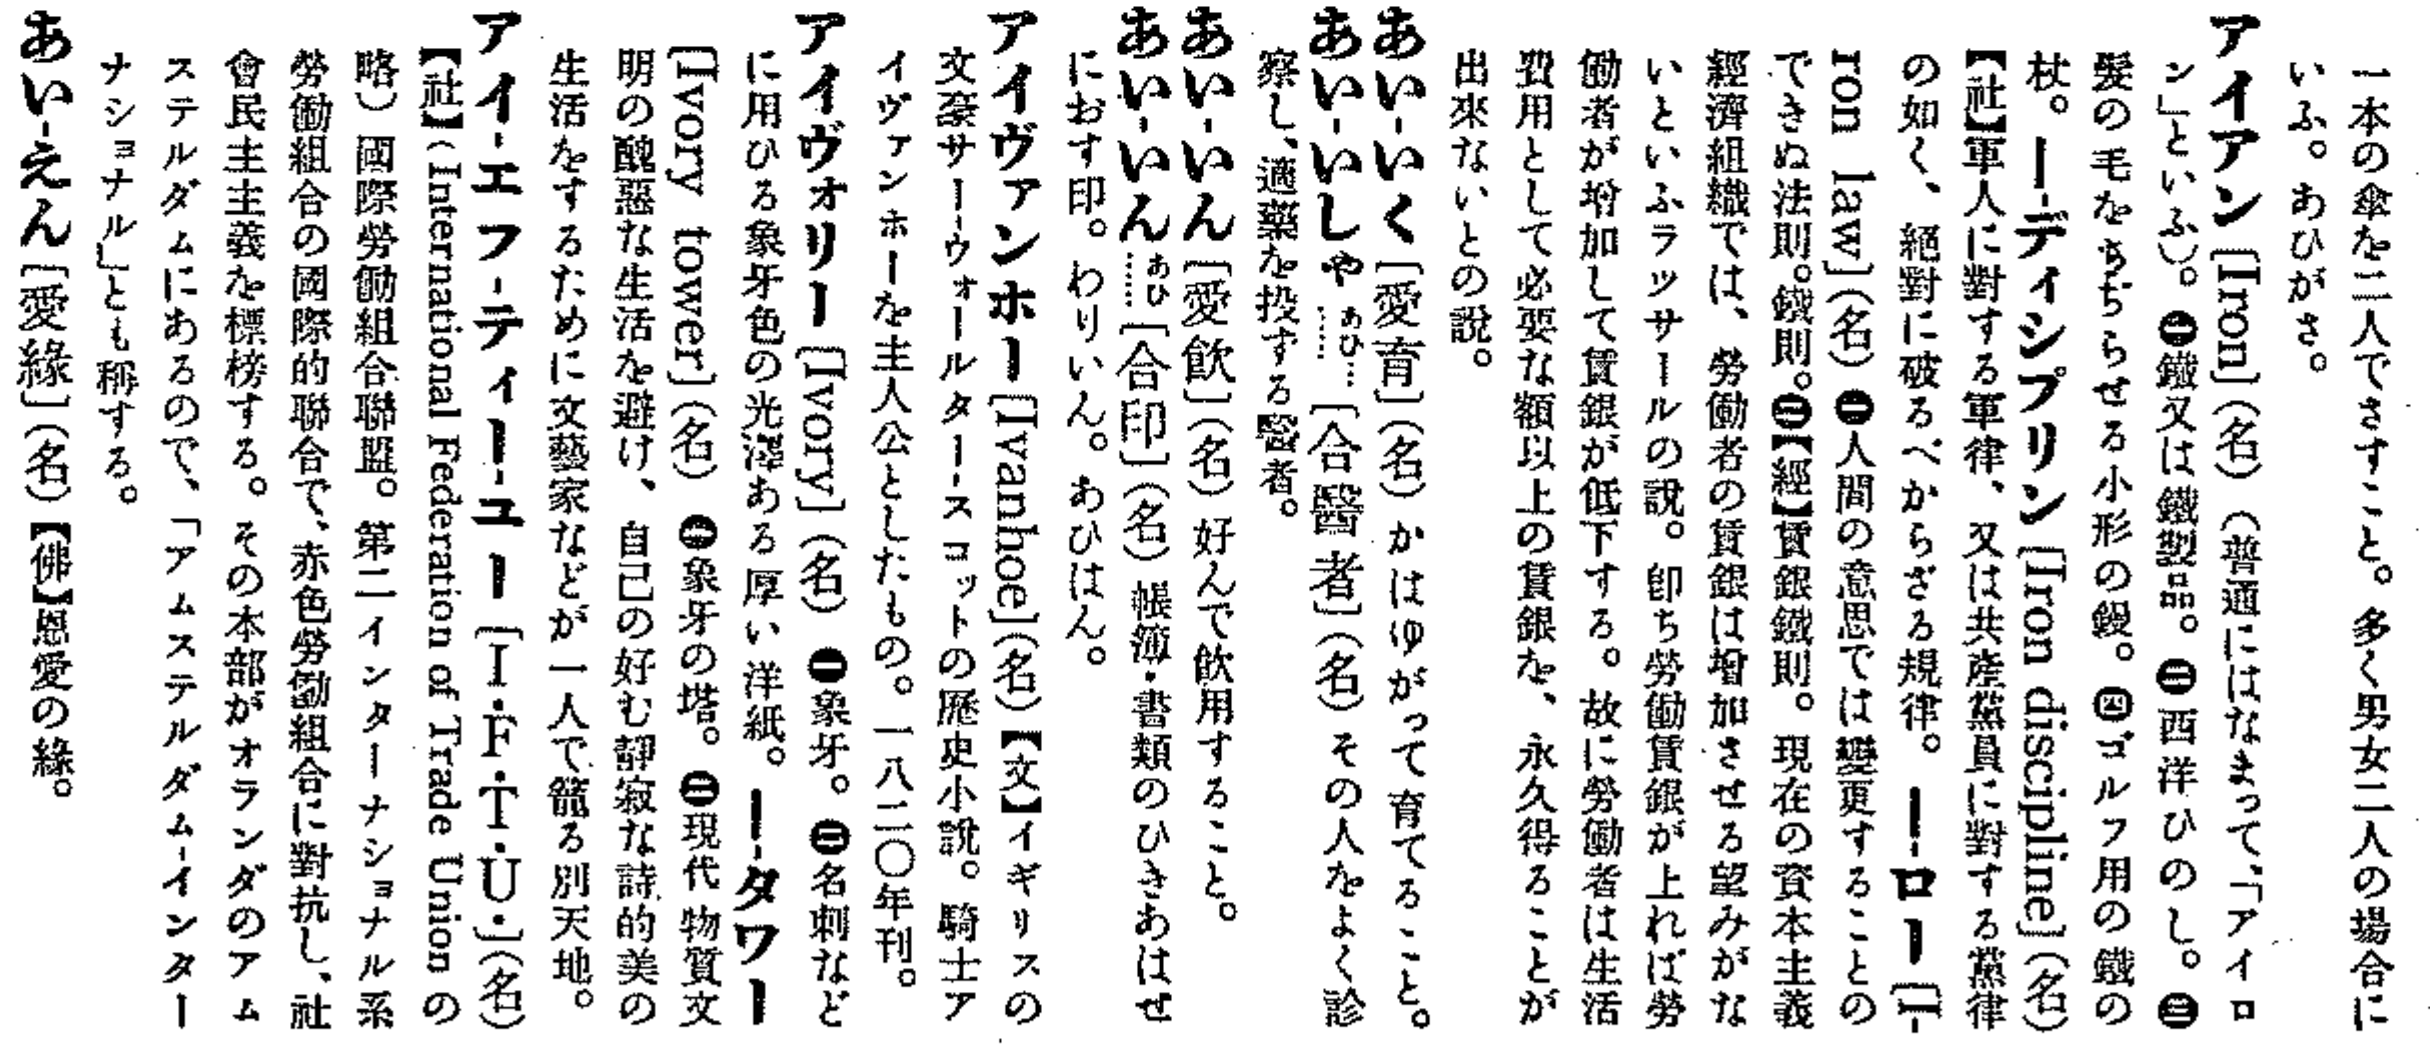
\includegraphics{https://raw.githubusercontent.com/RohanAlexander/japanese_dictionaries/master/inputs/cropped\%20pages/00-sample_pages_3_sec_1.png}
\textbf{Figure XX Section 1}

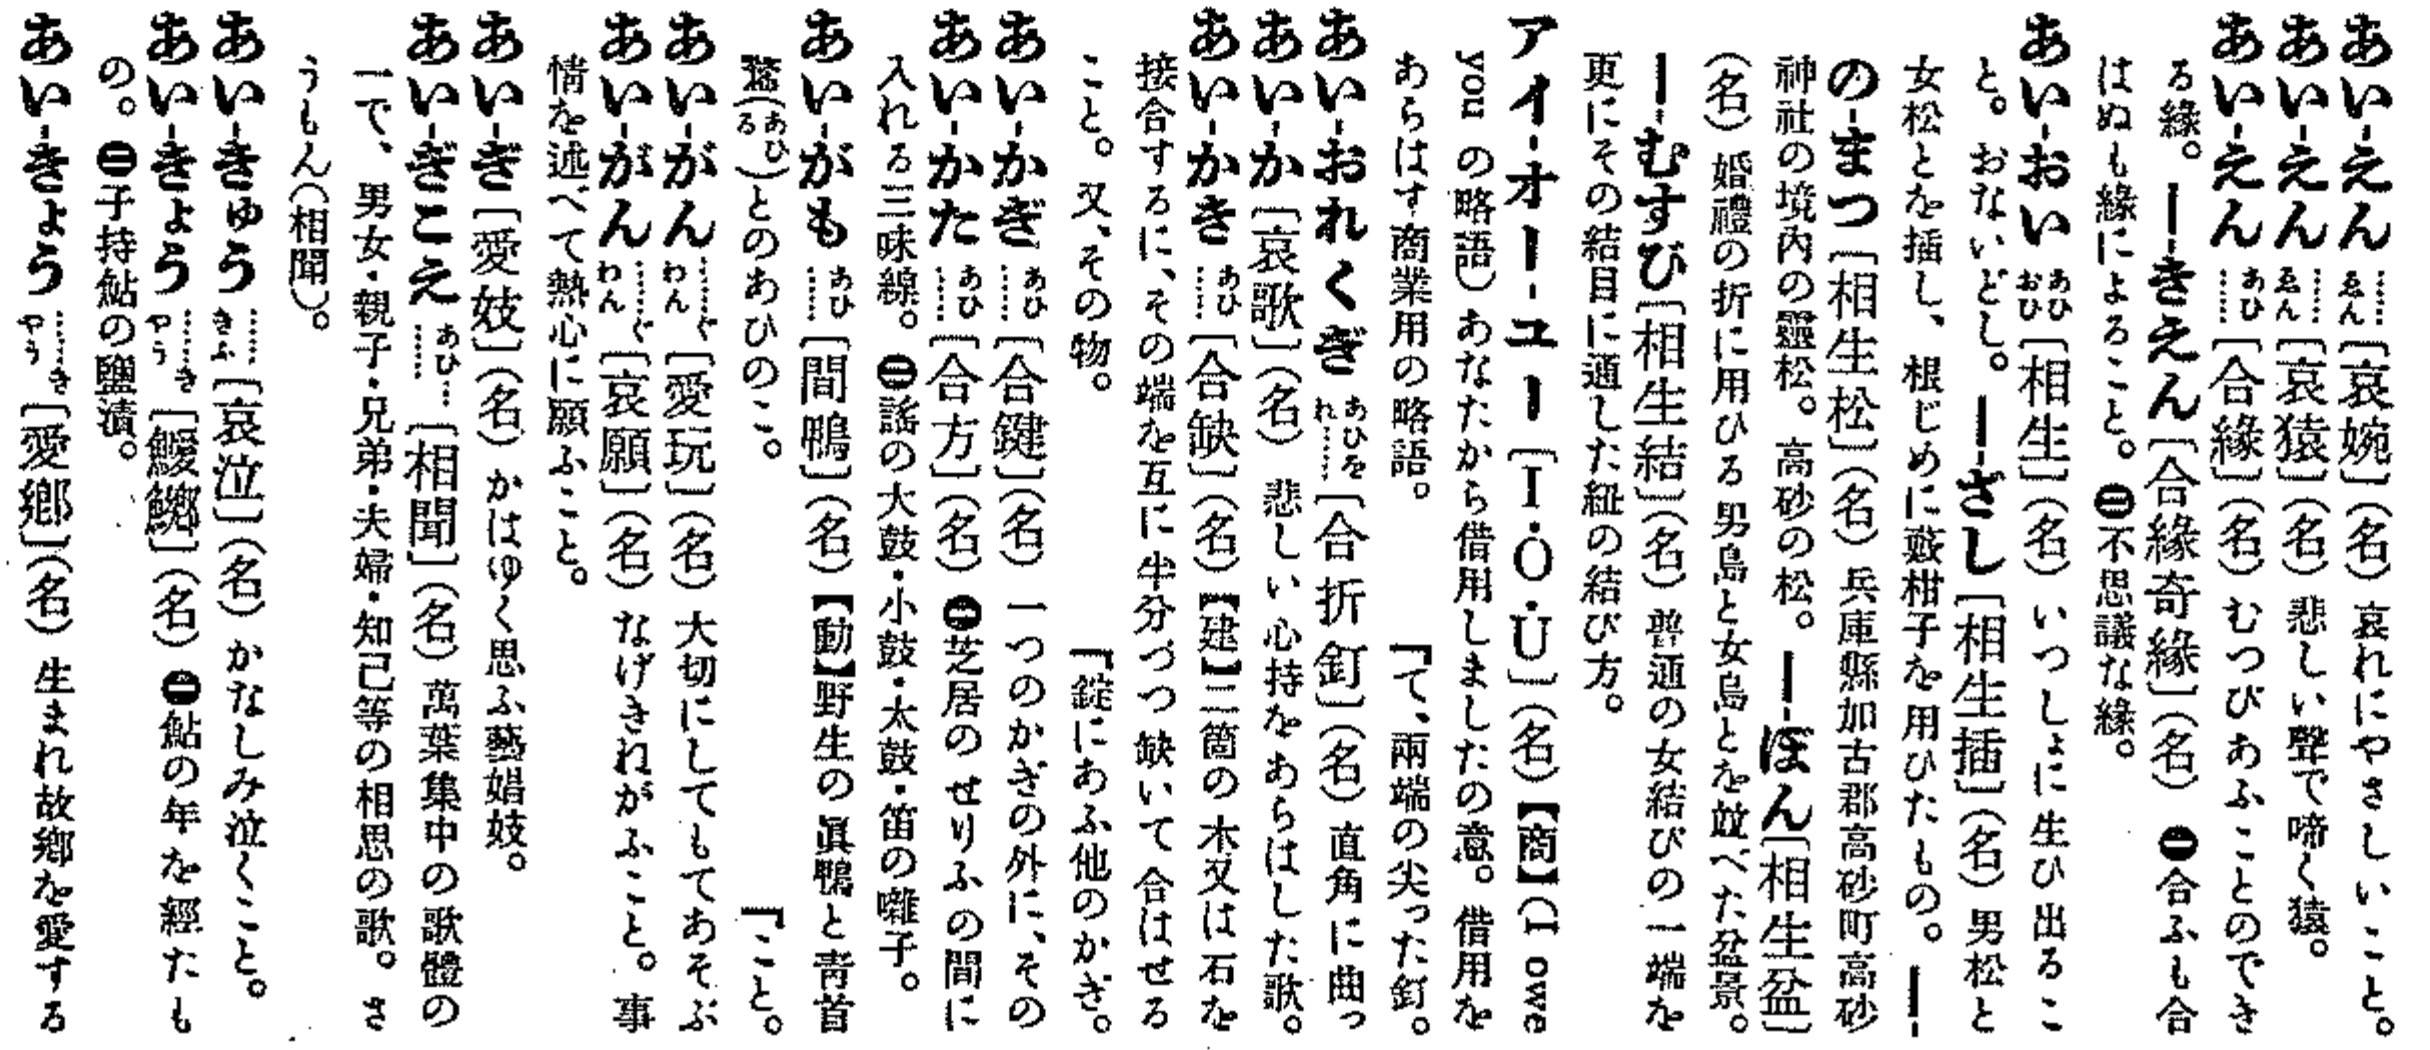
\includegraphics{https://raw.githubusercontent.com/RohanAlexander/japanese_dictionaries/master/inputs/cropped\%20pages/00-sample_pages_3_sec_2.png}
\textbf{Figure XX Section 2}

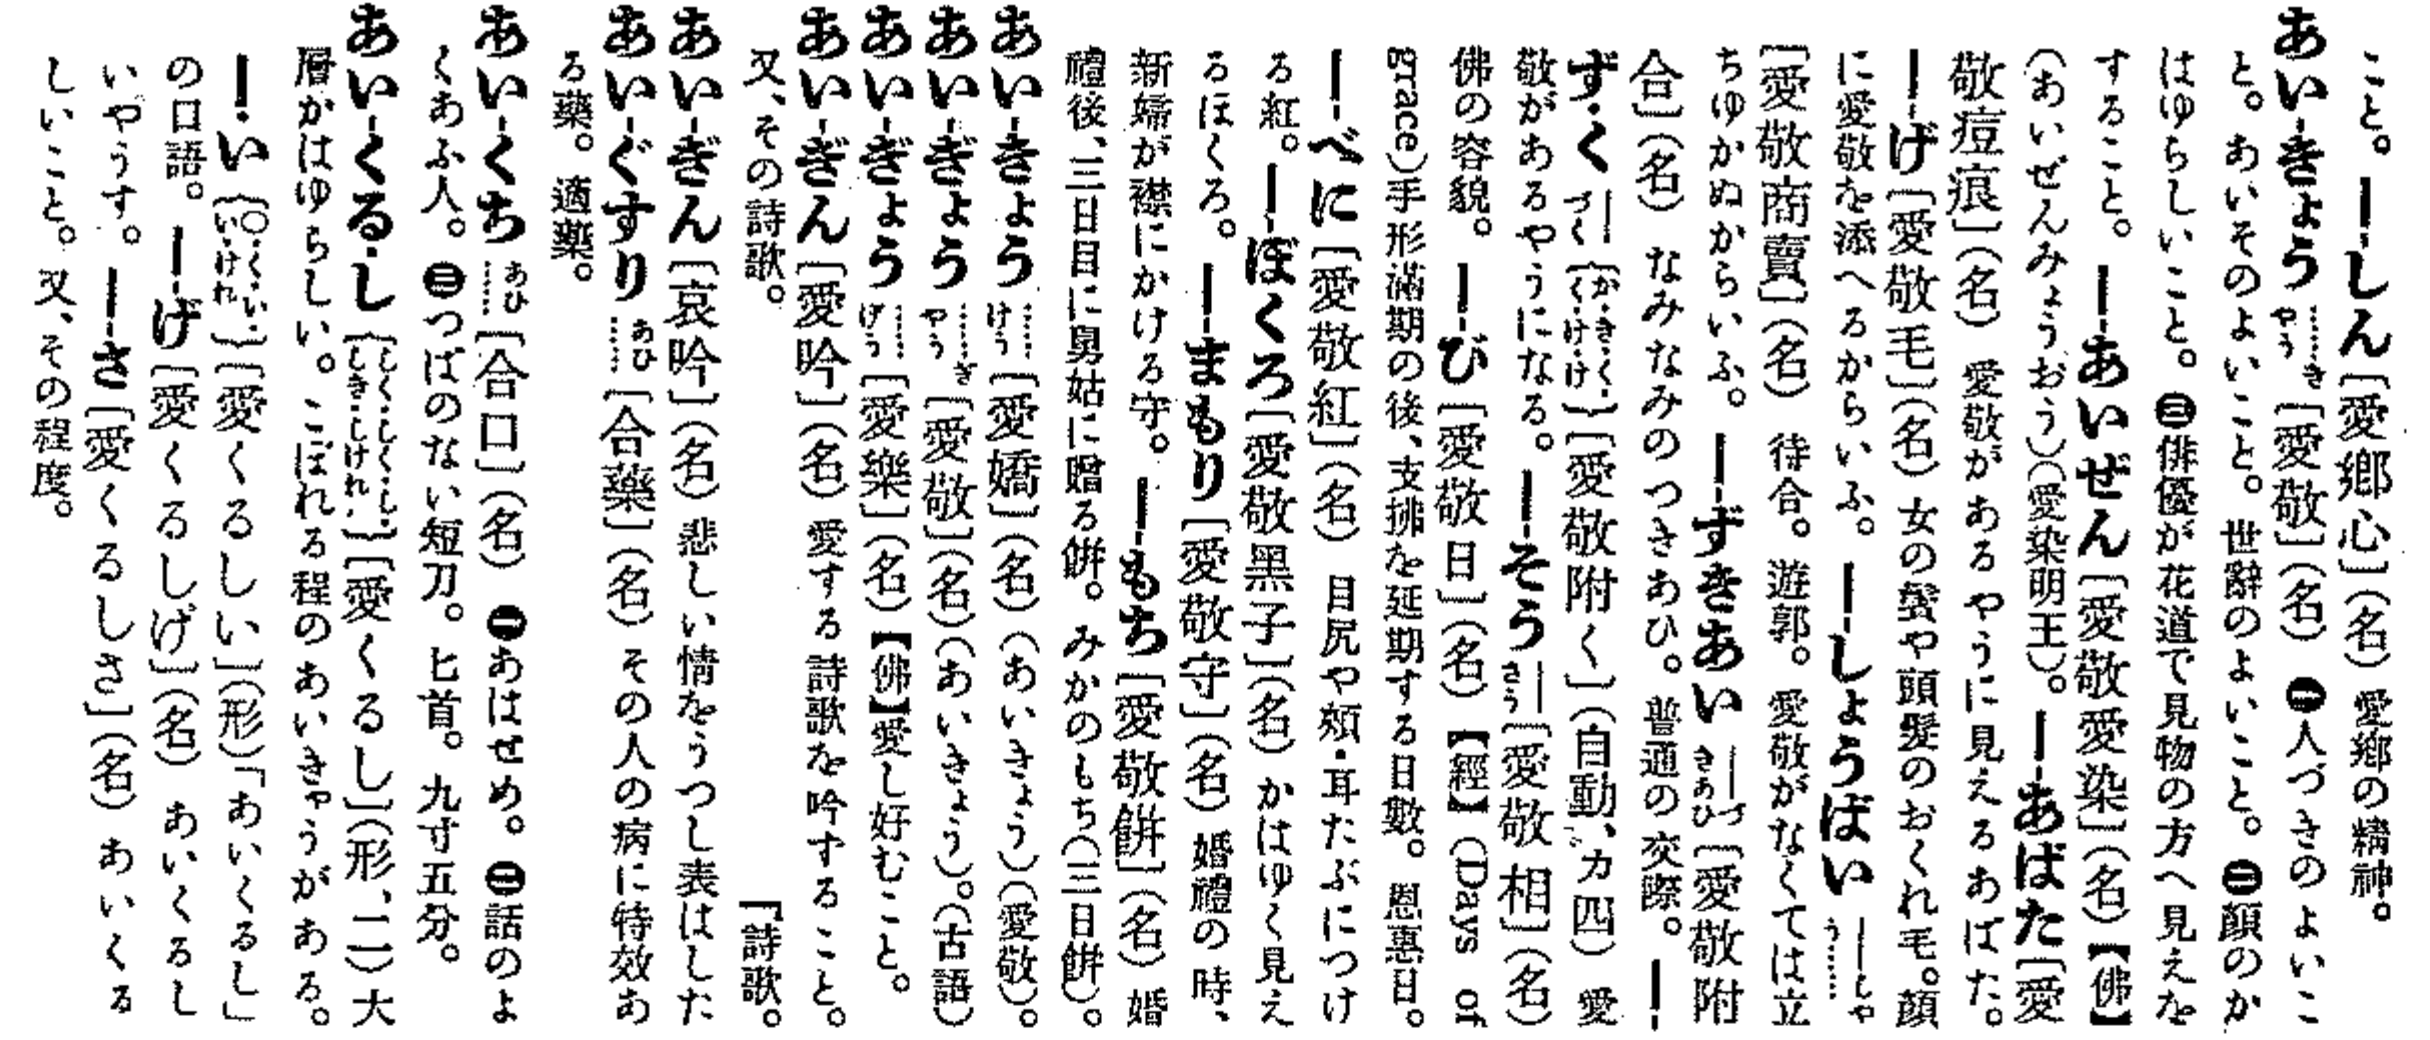
\includegraphics{https://raw.githubusercontent.com/RohanAlexander/japanese_dictionaries/master/inputs/cropped\%20pages/00-sample_pages_3_sec_3.png}
\textbf{Figure XX Section 3}

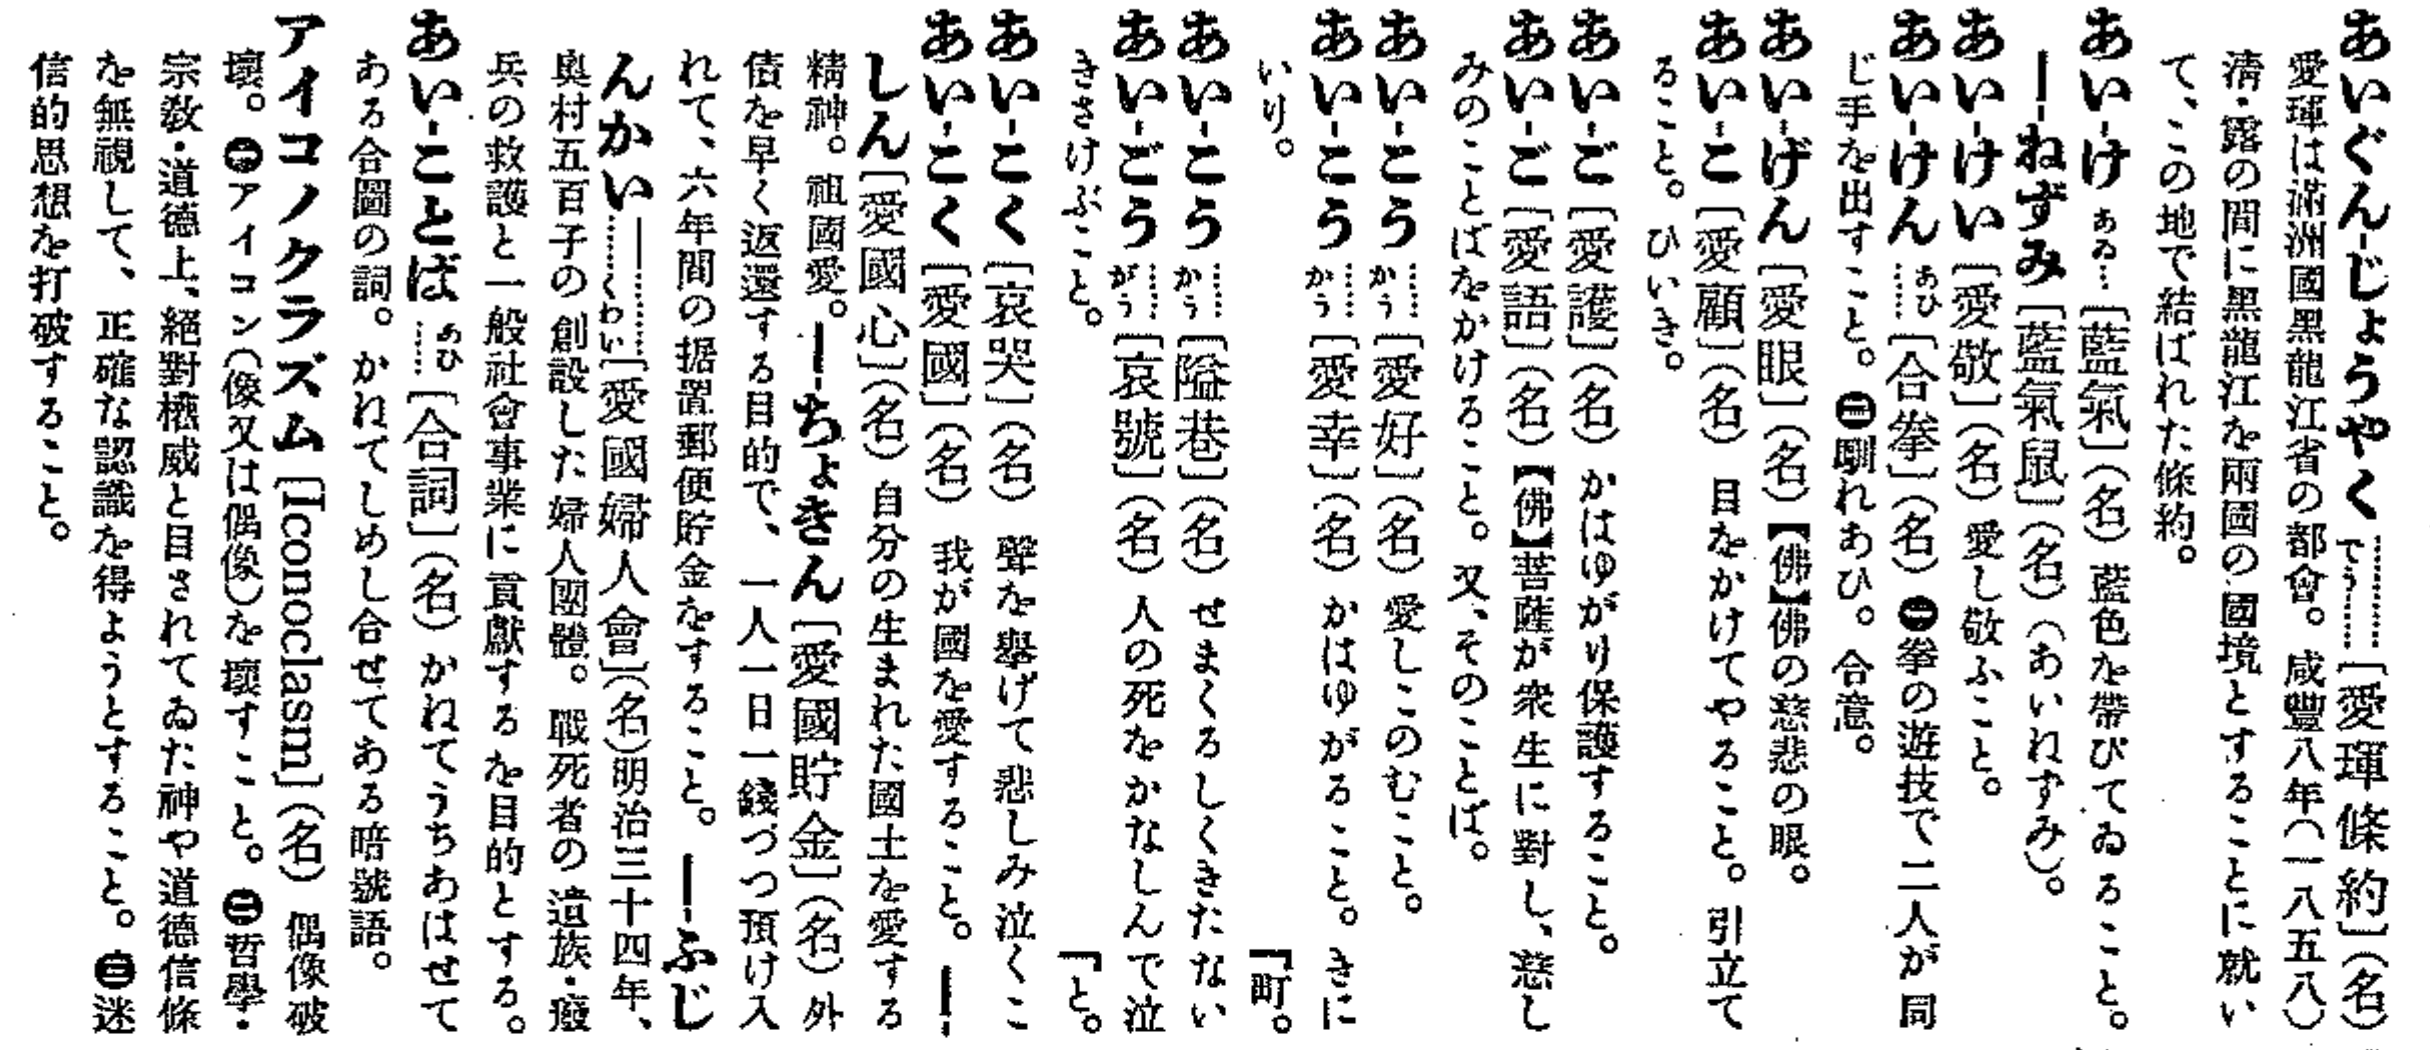
\includegraphics{https://raw.githubusercontent.com/RohanAlexander/japanese_dictionaries/master/inputs/cropped\%20pages/00-sample_pages_3_sec_4.png}
\textbf{Figure XX Section 4}

\hypertarget{ocr-options}{%
\subsection{OCR options}\label{ocr-options}}

The following list contains the OCR APIs and libraries available that
will be evaluated in this study:

\begin{longtable}[]{@{}lllll@{}}
\toprule
\begin{minipage}[b]{0.37\columnwidth}\raggedright
OCR Tool\strut
\end{minipage} & \begin{minipage}[b]{0.09\columnwidth}\raggedright
Company\strut
\end{minipage} & \begin{minipage}[b]{0.14\columnwidth}\raggedright
Type\strut
\end{minipage} & \begin{minipage}[b]{0.07\columnwidth}\raggedright
Monthly Price Aug/2020\strut
\end{minipage} & \begin{minipage}[b]{0.18\columnwidth}\raggedright
Tech Requierements\strut
\end{minipage}\tabularnewline
\midrule
\endhead
\begin{minipage}[t]{0.37\columnwidth}\raggedright
Azure Cognitive Services (OCR)\strut
\end{minipage} & \begin{minipage}[t]{0.09\columnwidth}\raggedright
Microsoft\strut
\end{minipage} & \begin{minipage}[t]{0.14\columnwidth}\raggedright
API\strut
\end{minipage} & \begin{minipage}[t]{0.07\columnwidth}\raggedright
Free Web Container: 5000/Free; S1 Web Container: 0-1M/\$1.50 per 1,000
trans, 1M-5M/\$1 per 1,000 trans, 5M-10M/\$0.65 per 1,000 trans,
10M-100M/\$0.65 per 1,000 trans, +100M/\$0.65 per 1,000 trans\strut
\end{minipage} & \begin{minipage}[t]{0.18\columnwidth}\raggedright
\strut
\end{minipage}\tabularnewline
\begin{minipage}[t]{0.37\columnwidth}\raggedright
Amazon Rekognition\strut
\end{minipage} & \begin{minipage}[t]{0.09\columnwidth}\raggedright
Amazon\strut
\end{minipage} & \begin{minipage}[t]{0.14\columnwidth}\raggedright
API\strut
\end{minipage} & \begin{minipage}[t]{0.07\columnwidth}\raggedright
First 1 million images: \$0.001 per image Next 9 million images \$0.0008
per image Next 90 million images \$0.0006 per image Over 100 million
images \$0.0004 per image\strut
\end{minipage} & \begin{minipage}[t]{0.18\columnwidth}\raggedright
\strut
\end{minipage}\tabularnewline
\begin{minipage}[t]{0.37\columnwidth}\raggedright
PyTesseract (Wrapper Google's OCR Engine)\strut
\end{minipage} & \begin{minipage}[t]{0.09\columnwidth}\raggedright
\strut
\end{minipage} & \begin{minipage}[t]{0.14\columnwidth}\raggedright
Python Library\strut
\end{minipage} & \begin{minipage}[t]{0.07\columnwidth}\raggedright
Free\strut
\end{minipage} & \begin{minipage}[t]{0.18\columnwidth}\raggedright
\strut
\end{minipage}\tabularnewline
\begin{minipage}[t]{0.37\columnwidth}\raggedright
Standard: \$0.002 per trans\strut
\end{minipage} & \begin{minipage}[t]{0.09\columnwidth}\raggedright
\strut
\end{minipage} & \begin{minipage}[t]{0.14\columnwidth}\raggedright
\strut
\end{minipage} & \begin{minipage}[t]{0.07\columnwidth}\raggedright
\strut
\end{minipage} & \begin{minipage}[t]{0.18\columnwidth}\raggedright
\strut
\end{minipage}\tabularnewline
\begin{minipage}[t]{0.37\columnwidth}\raggedright
Kraken (Linux OS)\strut
\end{minipage} & \begin{minipage}[t]{0.09\columnwidth}\raggedright
\strut
\end{minipage} & \begin{minipage}[t]{0.14\columnwidth}\raggedright
Python Library\strut
\end{minipage} & \begin{minipage}[t]{0.07\columnwidth}\raggedright
Free\strut
\end{minipage} & \begin{minipage}[t]{0.18\columnwidth}\raggedright
\strut
\end{minipage}\tabularnewline
\begin{minipage}[t]{0.37\columnwidth}\raggedright
Google Vision (for Text recognition)\strut
\end{minipage} & \begin{minipage}[t]{0.09\columnwidth}\raggedright
Google\strut
\end{minipage} & \begin{minipage}[t]{0.14\columnwidth}\raggedright
API\strut
\end{minipage} & \begin{minipage}[t]{0.07\columnwidth}\raggedright
1000/Free, 5 mill/\$1.5, \textgreater5mill/\$0.6\strut
\end{minipage} & \begin{minipage}[t]{0.18\columnwidth}\raggedright
\strut
\end{minipage}\tabularnewline
\begin{minipage}[t]{0.37\columnwidth}\raggedright
Amazon Textract\strut
\end{minipage} & \begin{minipage}[t]{0.09\columnwidth}\raggedright
Amazon\strut
\end{minipage} & \begin{minipage}[t]{0.14\columnwidth}\raggedright
API\strut
\end{minipage} & \begin{minipage}[t]{0.07\columnwidth}\raggedright
First 1 Million pages: \$0.015 - \$0.05 per page, Over 1 Million pages:
\$0.01 - \$0.04 per page\strut
\end{minipage} & \begin{minipage}[t]{0.18\columnwidth}\raggedright
\strut
\end{minipage}\tabularnewline
\begin{minipage}[t]{0.37\columnwidth}\raggedright
Kindai-OCR\strut
\end{minipage} & \begin{minipage}[t]{0.09\columnwidth}\raggedright
Result of n2i Project\strut
\end{minipage} & \begin{minipage}[t]{0.14\columnwidth}\raggedright
Python Library\strut
\end{minipage} & \begin{minipage}[t]{0.07\columnwidth}\raggedright
Free\strut
\end{minipage} & \begin{minipage}[t]{0.18\columnwidth}\raggedright
\strut
\end{minipage}\tabularnewline
\bottomrule
\end{longtable}

\hypertarget{azure-corgnitive-services---computer-vision-ocr}{%
\subsection{Azure Corgnitive Services - Computer Vision
OCR}\label{azure-corgnitive-services---computer-vision-ocr}}

Among the Microsoft Azure's portfolio, Azure Cognitive Services offers
Computer Vision, an API that processes images and returns information
based on the visual features the user is interested in. Those services
comprise object detection of an image, visual features tagging, image
categorization, Optical Character Recognition (OCR), among \(others^4\).
The OCR API processes an image and returns the language of the document,
orientation, regions, lines, and finally, the characters.

In python we need several libraries for calling the API.

\begin{Shaded}
\begin{Highlighting}[]
\ImportTok{import}\NormalTok{ os}
\ImportTok{import}\NormalTok{ sys}
\ImportTok{import}\NormalTok{ requests}
\CommentTok{# If you are using a Jupyter notebook, uncomment the following line.}
\CommentTok{#%matplotlib inline}
\ImportTok{import}\NormalTok{ matplotlib.pyplot }\ImportTok{as}\NormalTok{ plt}
\ImportTok{from}\NormalTok{ matplotlib.patches }\ImportTok{import}\NormalTok{ Rectangle}
\ImportTok{from}\NormalTok{ PIL }\ImportTok{import}\NormalTok{ Image}
\ImportTok{from}\NormalTok{ io }\ImportTok{import}\NormalTok{ BytesIO}
\ImportTok{import}\NormalTok{ matplotlib}
\ImportTok{from}\NormalTok{ os }\ImportTok{import}\NormalTok{ path}
\ImportTok{import}\NormalTok{ ast}
\end{Highlighting}
\end{Shaded}

Then, we need to create headers and parameters necessary for calling the
API. The library \textbf{requests} is commonly used in python to do
that. The method \textbf{post} is needed as the API uses the HTTP method
POST.

\begin{Shaded}
\begin{Highlighting}[]
\CommentTok{#Create the URL for the API call. The endpoint corresponds to the Azure's }
\CommentTok{# endpoint of the account.}
\NormalTok{ocr_url }\OperatorTok{=}\NormalTok{ endpoint }\OperatorTok{+} \StringTok{"vision/v3.0/ocr"} 

\CommentTok{#Create the header using the Azure's subscription key.}
\NormalTok{headers }\OperatorTok{=}\NormalTok{ \{}\StringTok{'Ocp-Apim-Subscription-Key'}\NormalTok{: subscription_key\} }

\CommentTok{#In params language': 'ja' for japanese only. 'unk' means self detection }
\NormalTok{params }\OperatorTok{=}\NormalTok{ \{}\StringTok{'language'}\NormalTok{: }\StringTok{'unk'}\NormalTok{, }\StringTok{'detectOrientation'}\NormalTok{: }\StringTok{'true'}\NormalTok{\} }
\NormalTok{data }\OperatorTok{=}\NormalTok{ \{}\StringTok{'url'}\NormalTok{: image_url\}}

\CommentTok{#Call and save the response using the method post from the library request}
\NormalTok{response }\OperatorTok{=}\NormalTok{ requests.post(ocr_url, headers}\OperatorTok{=}\NormalTok{headers, params}\OperatorTok{=}\NormalTok{params, json}\OperatorTok{=}\NormalTok{data)}
\end{Highlighting}
\end{Shaded}

Here we have an example of the response:

\begin{verbatim}
{'language': 'ja',
 'textAngle': 0.0,
 'orientation': 'Up',
 'regions': [{'boundingBox': '31,30,1521,2721',
   'lines': [{'boundingBox': '730,30,44,2718',
     'words': [{'boundingBox': '735,30,34,34', 'text': 'あ'},
      {'boundingBox': '736,71,34,26', 'text': 'い'},
      {'boundingBox': '749,100,6,11', 'text': '・'},
      {'boundingBox': '735,116,34,27', 'text': 'い'},
      {'boundingBox': '736,149,33,33', 'text': 'ん'},
\end{verbatim}

\hypertarget{language-and-orientation}{%
\subsubsection{Language and
Orientation}\label{language-and-orientation}}

Figure 1 presents a sample that corresponds to the section 1 of the
image containing Japanese text, but it also contains English text in
some fragments of the text. The API offers the possibility to do
self-detection, which in this case is helpful, but also the opportunity
to specify the language in advance. Moreover, the orientation can also
be self-detected or not.

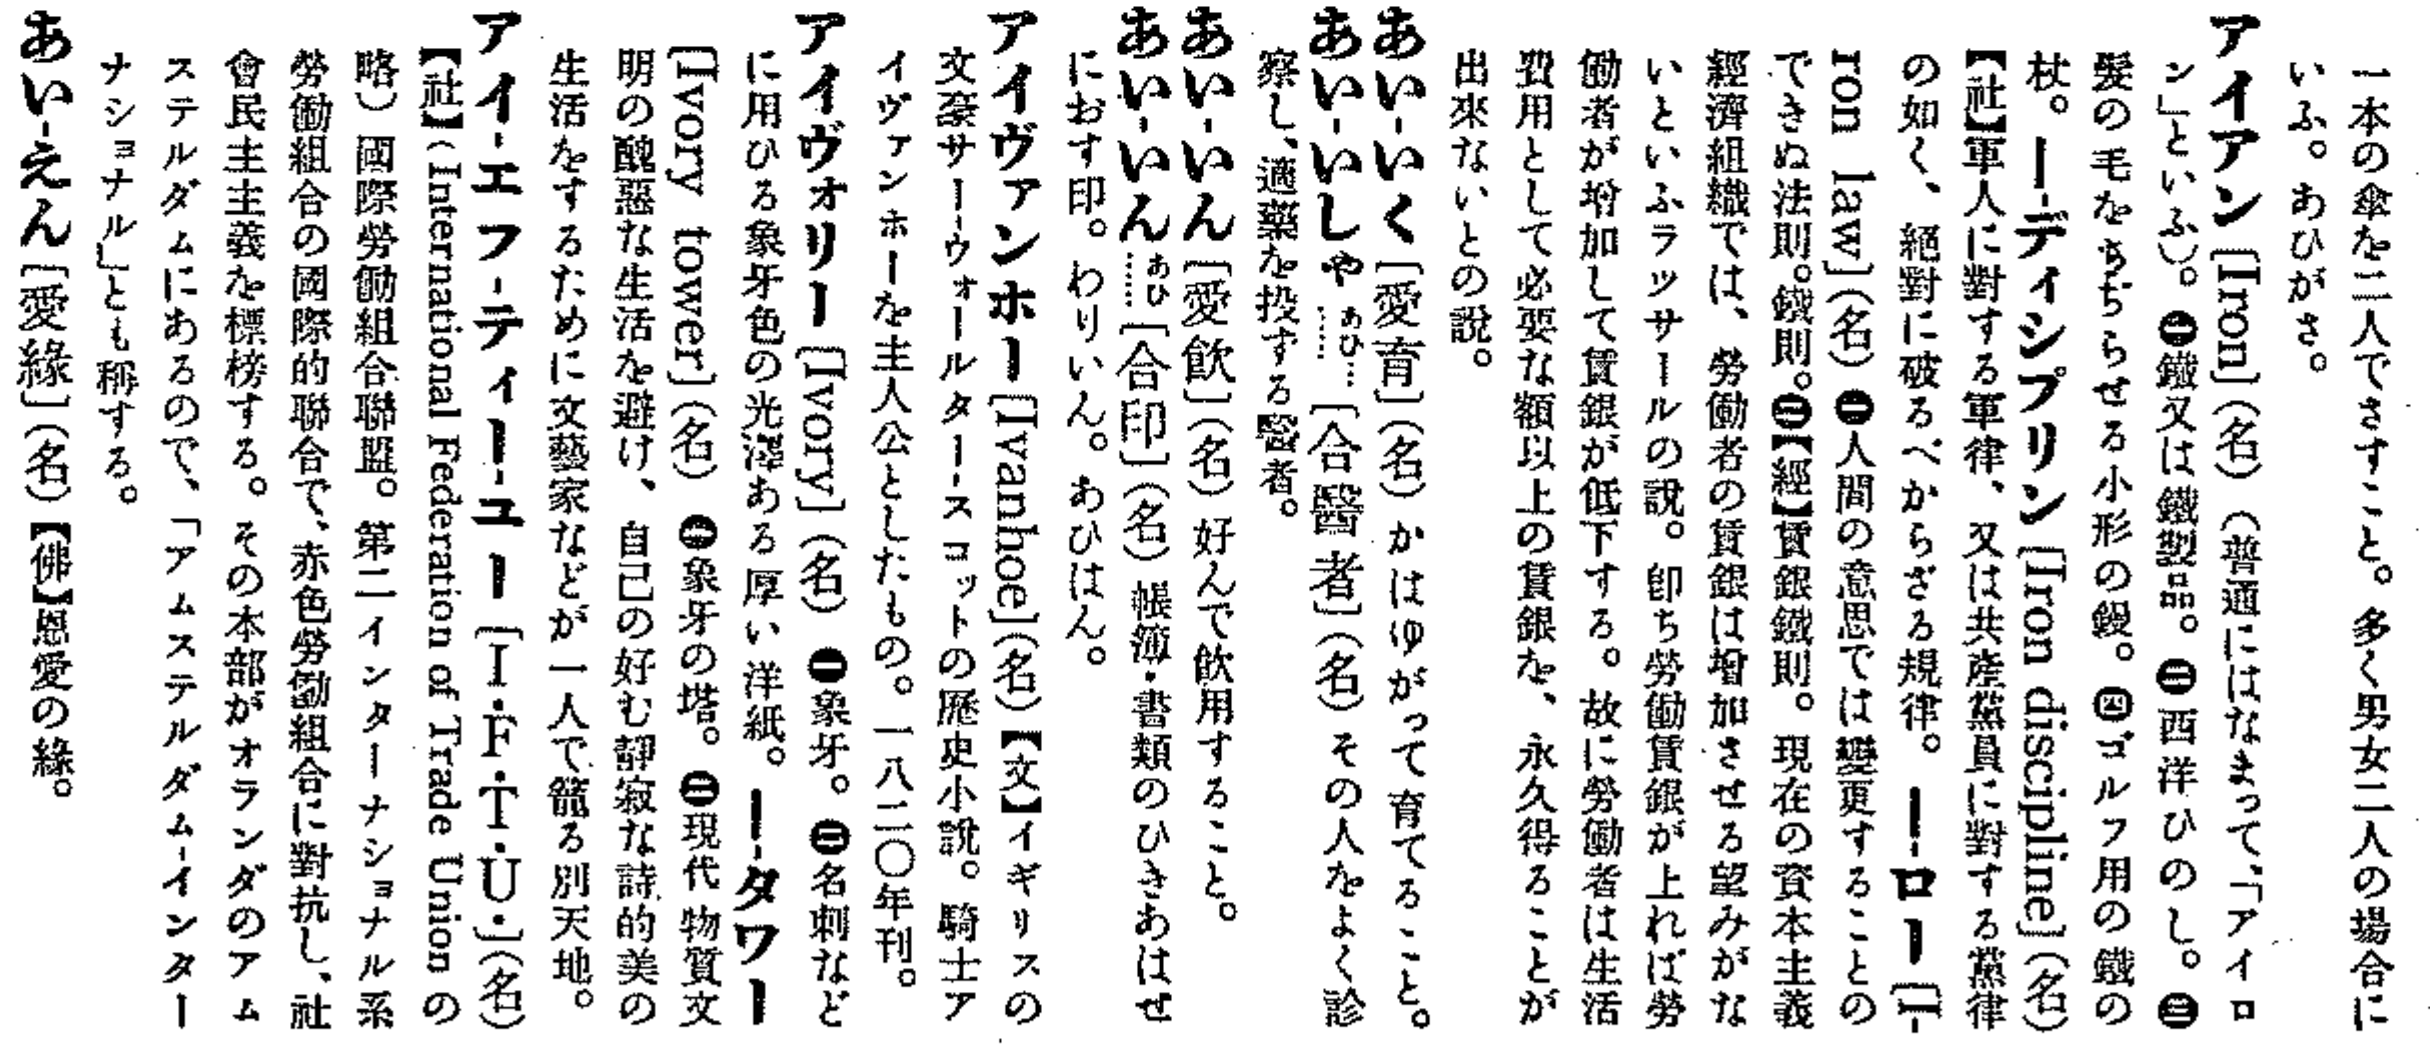
\includegraphics{E:/Users/Usuario/Documents/GitHub_Website/website/japanese_dictionaries/outputs/documents/azure-images/section1.png}
\textbf{Figure 1}

\hypertarget{regions}{%
\subsubsection{Regions}\label{regions}}

The blue line figure 2 denotes the segment from the image that includes
the characters. In this example, there is only one blue line because the
document is only text. In other cases, it may contain images requiring
more than one region.

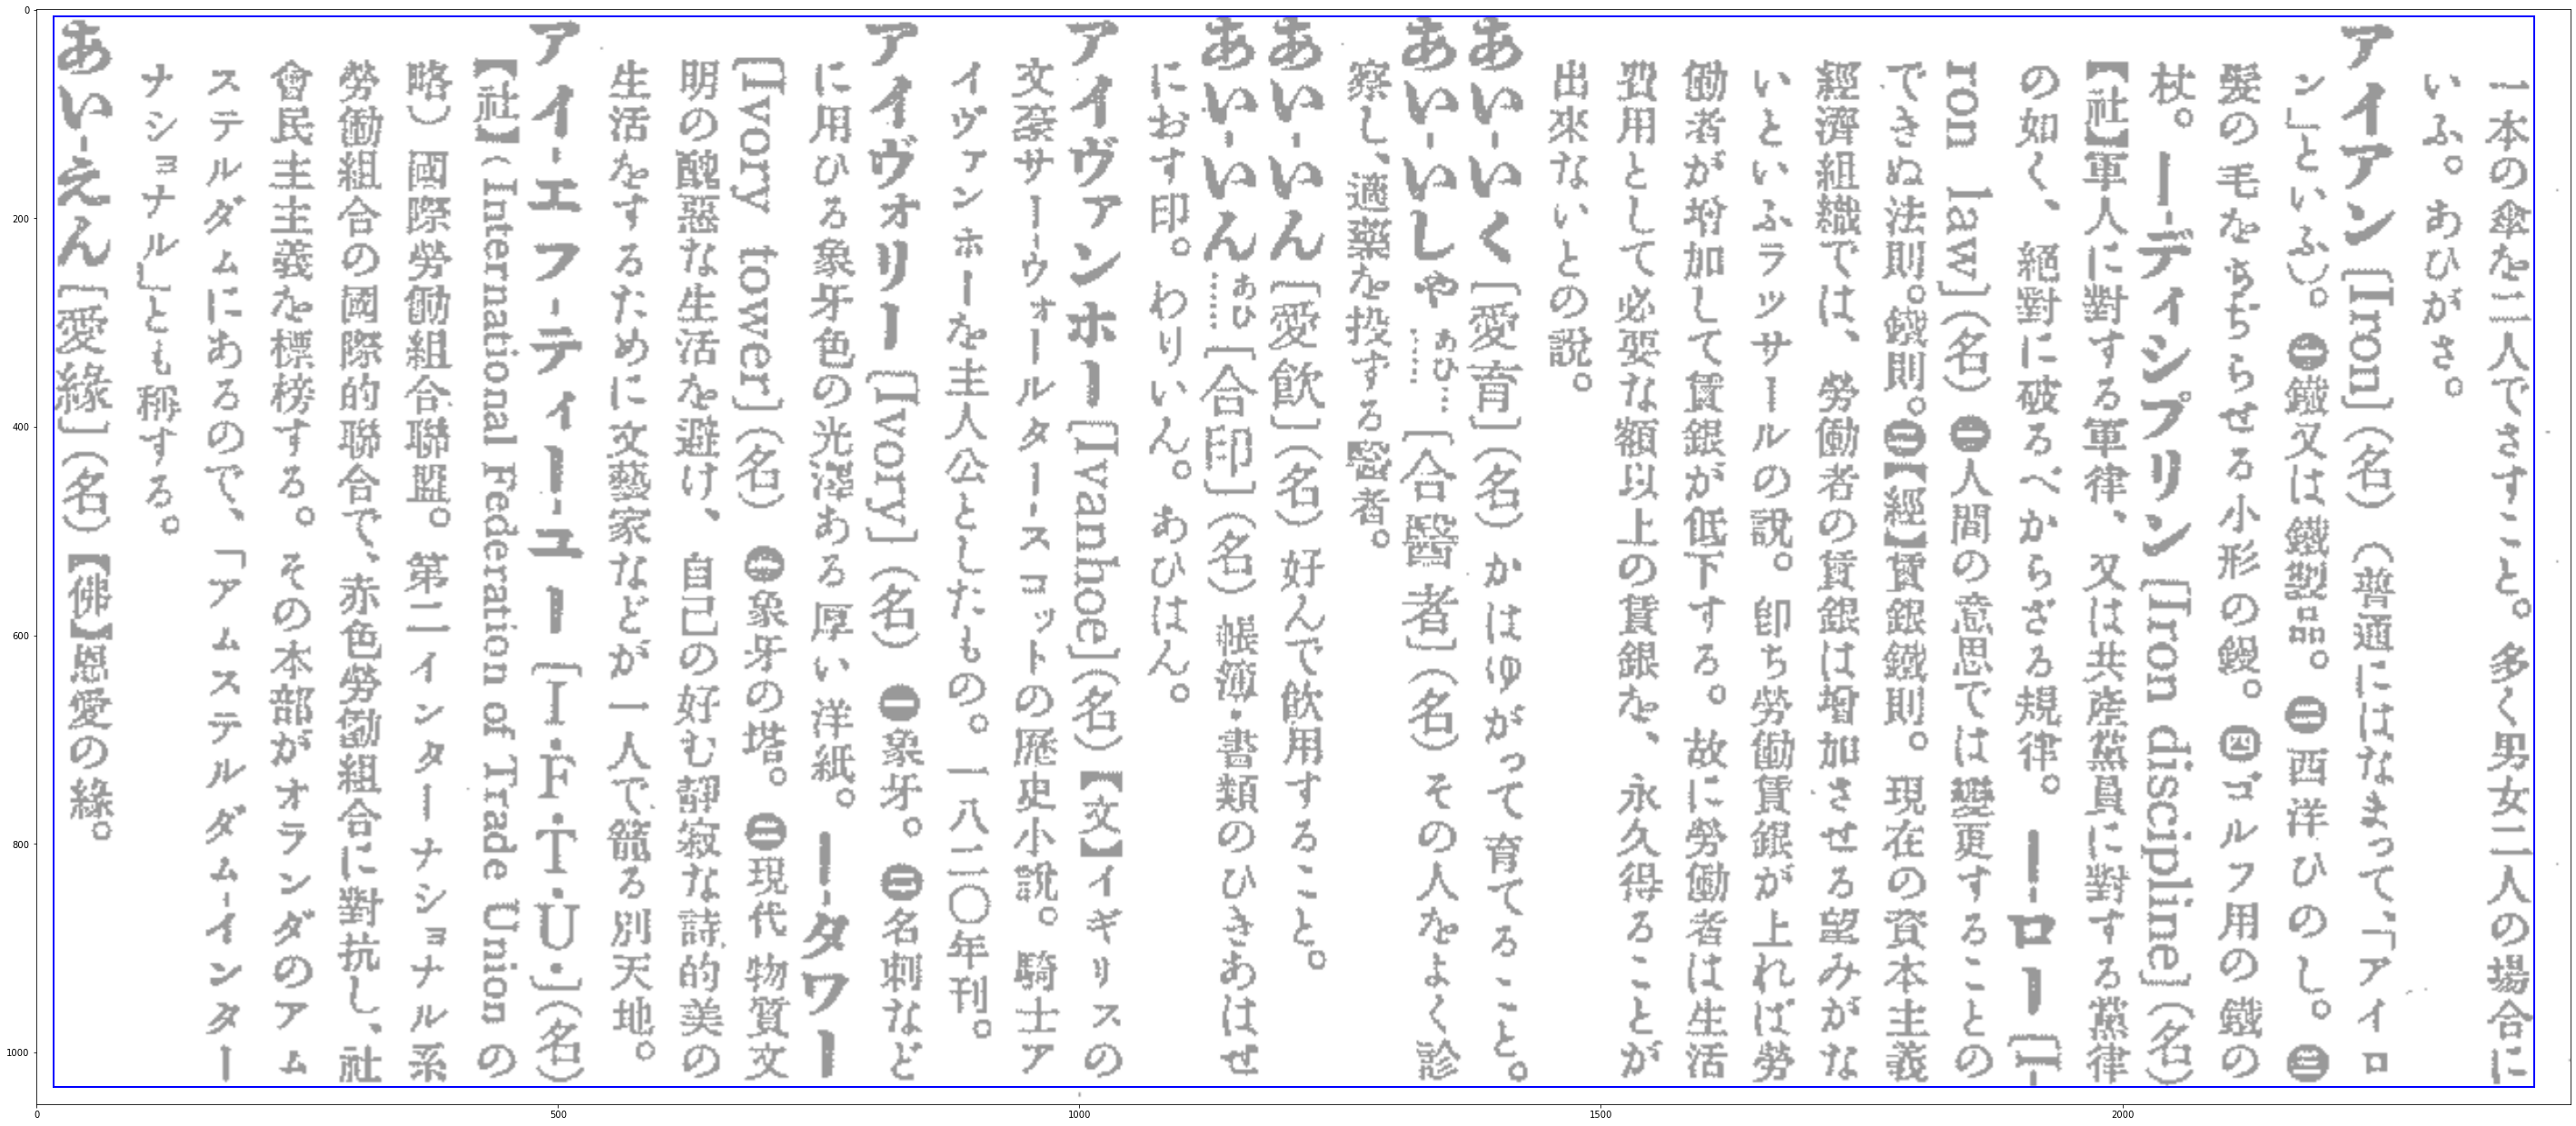
\includegraphics{E:/Users/Usuario/Documents/GitHub_Website/website/japanese_dictionaries/outputs/documents/azure-images/region-section1.png}
\textbf{Figure 2}

\hypertarget{lines}{%
\subsubsection{Lines}\label{lines}}

Once the region is defined, the API provides in figure 3 (red
rectangles) the subsets of characters of the region called Lines. From
the example, we can see that some characters are not included in any of
the lines. Those characters are not recognized by the API.

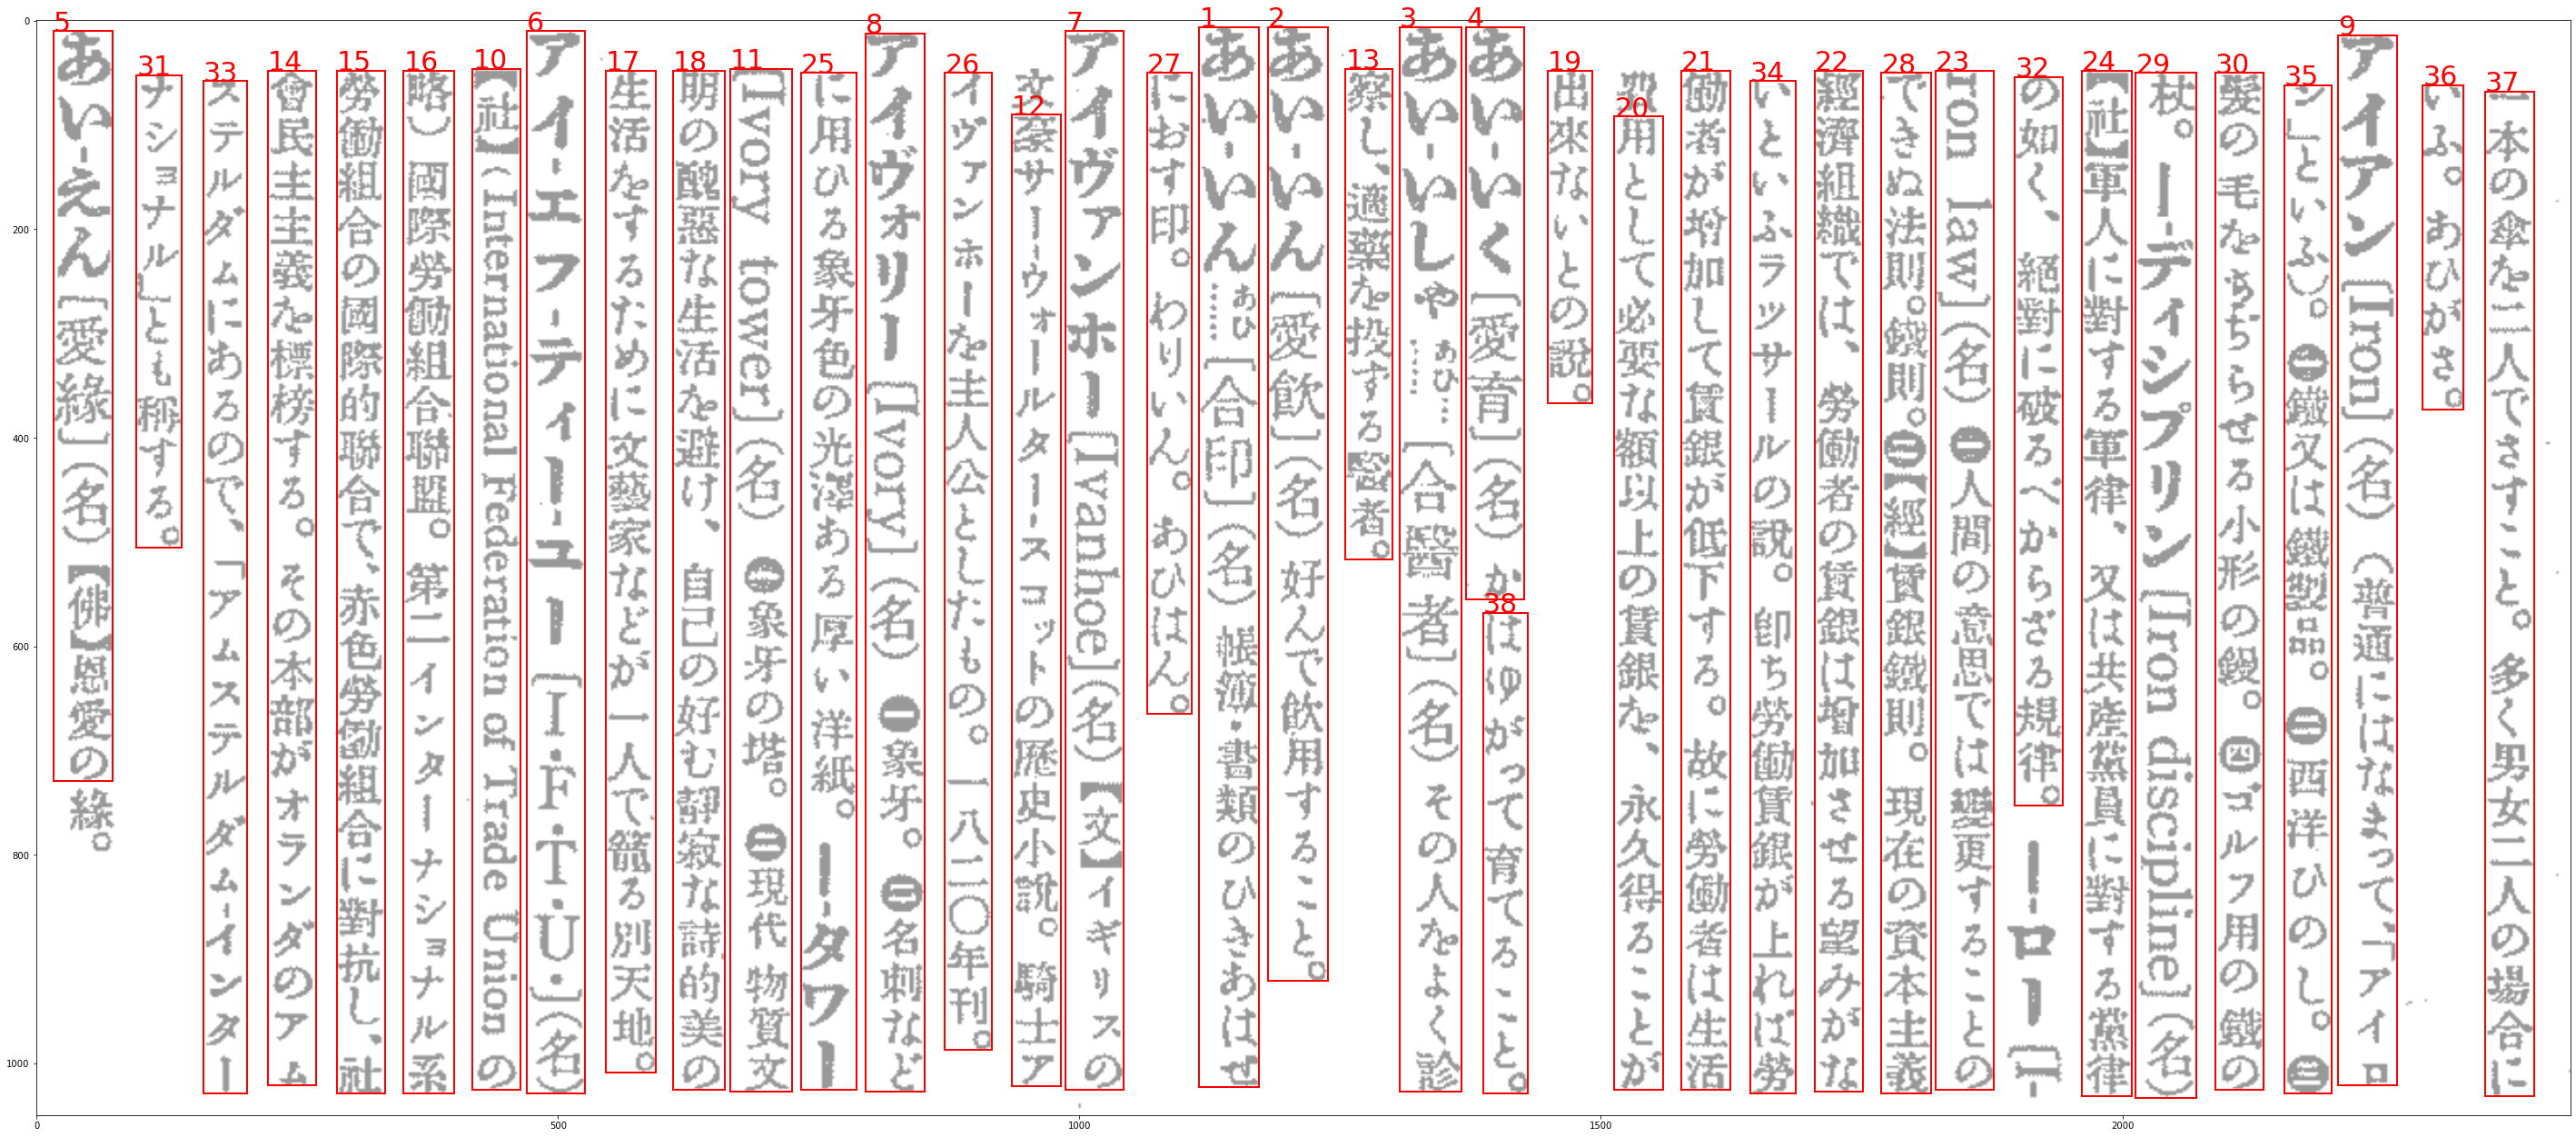
\includegraphics{E:/Users/Usuario/Documents/GitHub_Website/website/japanese_dictionaries/outputs/documents/azure-images/lines-section1.png}\\
\textbf{Figure 3}

\hypertarget{the-character-boundaries}{%
\subsubsection{The Character
Boundaries}\label{the-character-boundaries}}

After the lines are identified, the API provides in figure 4 each
recognized character bounding boxes. Those without a yellow square were
not recognized by the API in this example.

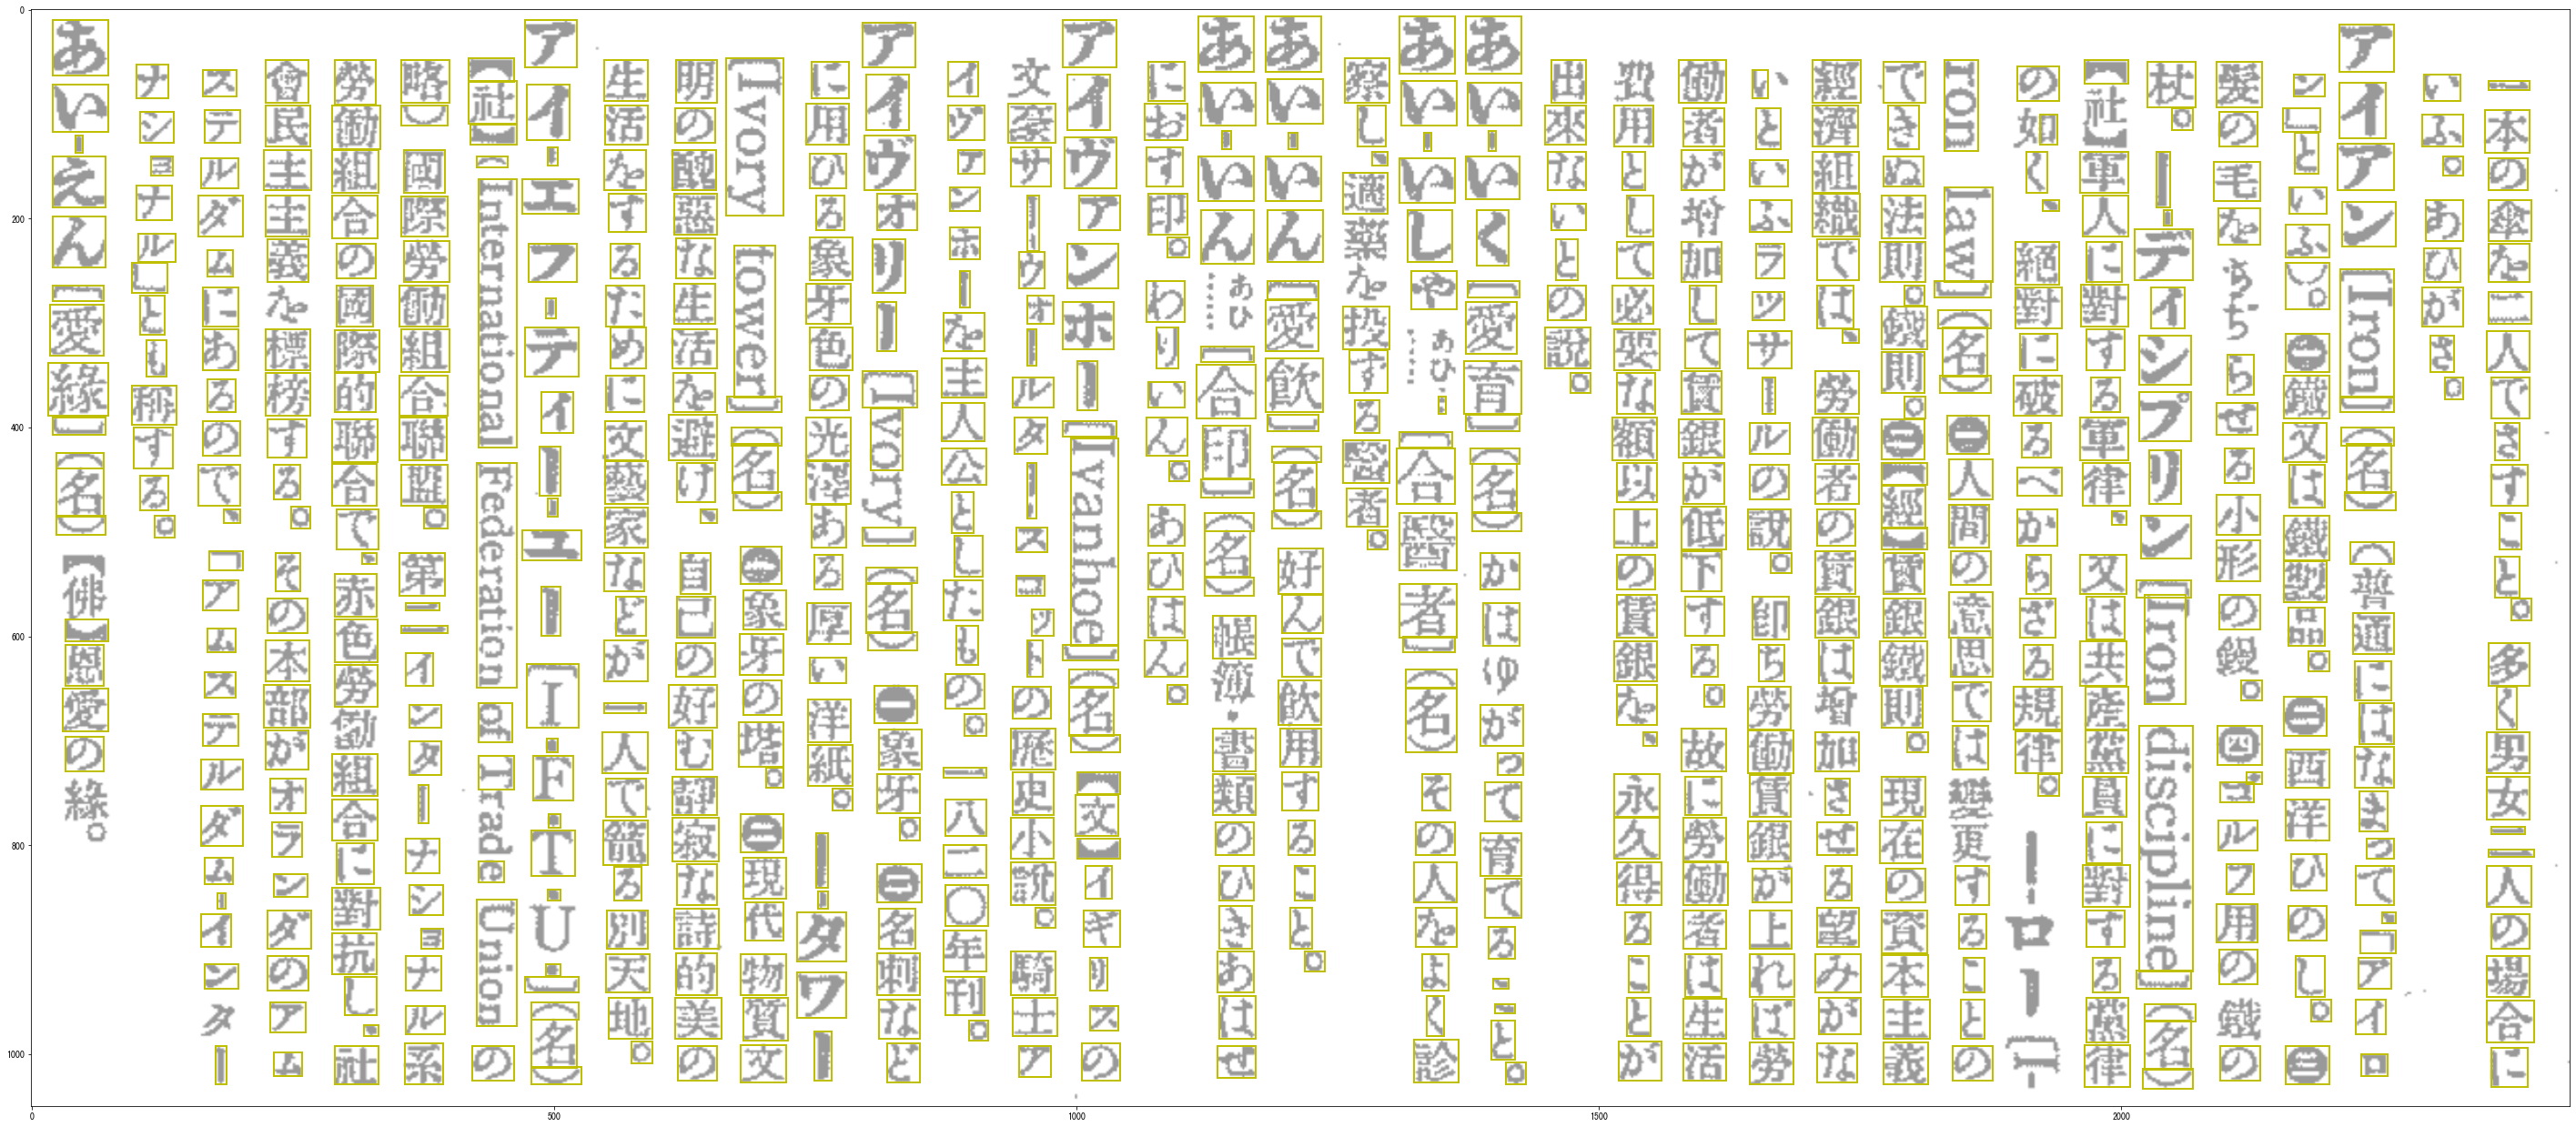
\includegraphics{E:/Users/Usuario/Documents/GitHub_Website/website/japanese_dictionaries/outputs/documents/azure-images/boundaries-section1.png}
\textbf{Figure 4}

\hypertarget{characters}{%
\subsubsection{Characters}\label{characters}}

Once the bounding boxes are located, each character takes its
corresponding place, as it is shown in figure 5.

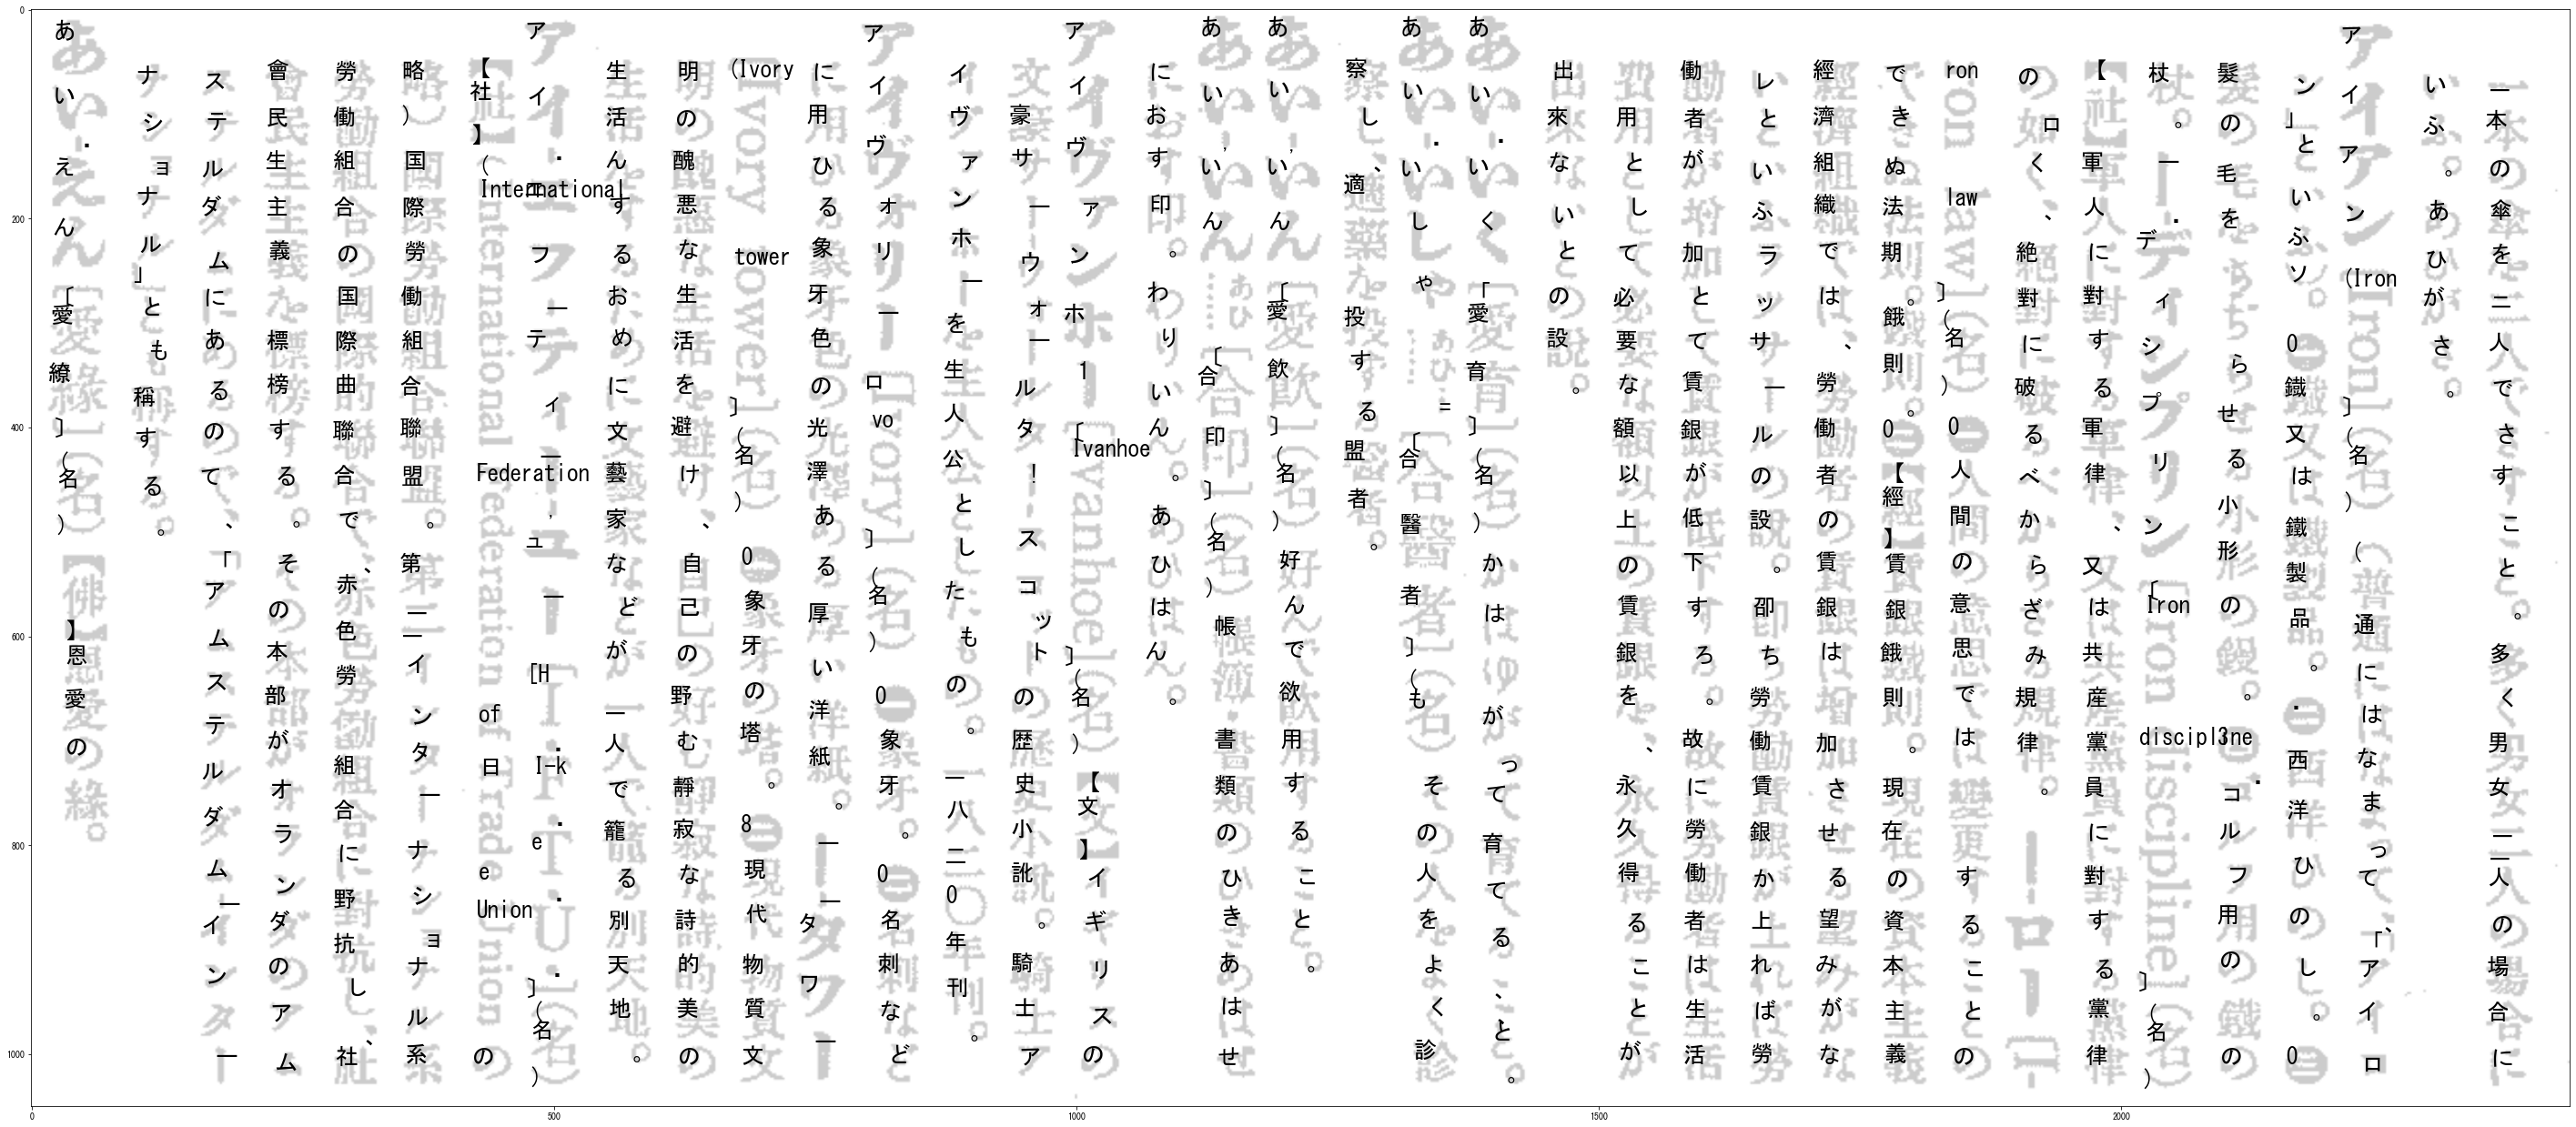
\includegraphics{E:/Users/Usuario/Documents/GitHub_Website/website/japanese_dictionaries/outputs/documents/azure-images/characters-section1.png}
\textbf{Figure 5}

\hypertarget{advantages-and-disadvantages}{%
\subsubsection{Advantages and
Disadvantages}\label{advantages-and-disadvantages}}

\hypertarget{advantages}{%
\paragraph{Advantages}\label{advantages}}

The API is easy to use after reading the documentation. It offers an
example of how to use it in different programming languages. It also
offers the possibility to self-detect languages and the orientation of
the document. The response is clear, and extract the information from
the JSON file is not complicated.

\hypertarget{disadvantages}{%
\paragraph{Disadvantages}\label{disadvantages}}

Even though the API offers the possibility to self-detect the language,
It changes the order in which the characters should be in the output. In
figures 6 we can see that the first line provided by the self-detection
approach is located in the middle. This situation does not allow a
correct interpretation of the text because it does not follow the
reading pattern. In this case, it is a vertical orientation, which means
we have to read it from right to left.

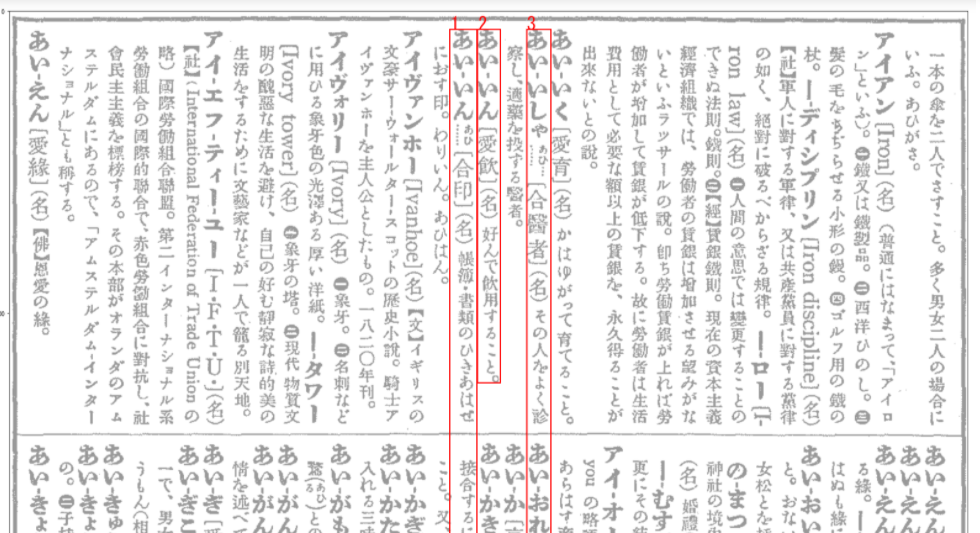
\includegraphics{E:/Users/Usuario/Documents/GitHub_Website/website/japanese_dictionaries/outputs/documents/azure-images/self-detection.png}
\textbf{Figure 6}

When the parameter language is stated as Japanese since the beginning,
as we can see in figure 7, it recognizes the first line correctly.

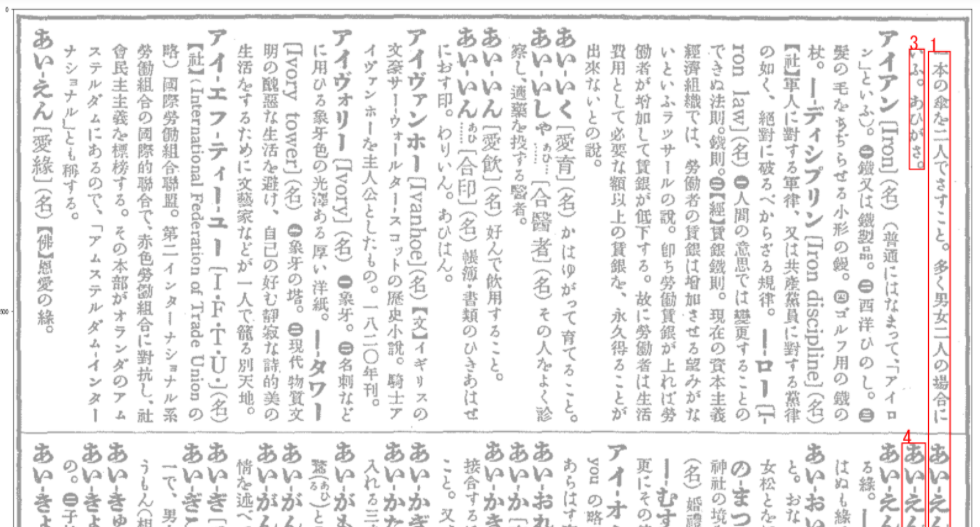
\includegraphics{E:/Users/Usuario/Documents/GitHub_Website/website/japanese_dictionaries/outputs/documents/azure-images/japanese-parameter.png}
\textbf{Figure 7}

\hypertarget{google-vision-ocr}{%
\subsection{Google Vision OCR}\label{google-vision-ocr}}

Google Vision API can integrate vision detection features, including
image labeling, face and landmark detection, optical character
recognition (OCR), and tagging of explicit content. The text recognition
process detects text in images and recognizes the text contained
therein. Once detected, the recognizer then determines the actual text
in each block and segments it into lines and words.

To evaluate this OCR option, we need the following python libraries.

\begin{Shaded}
\begin{Highlighting}[]
\ImportTok{from}\NormalTok{ os }\ImportTok{import}\NormalTok{ path}
\ImportTok{from}\NormalTok{ PIL }\ImportTok{import}\NormalTok{ Image}
\ImportTok{from}\NormalTok{ PIL }\ImportTok{import}\NormalTok{ ImageFont}
\ImportTok{from}\NormalTok{ PIL }\ImportTok{import}\NormalTok{ ImageDraw}
\ImportTok{from}\NormalTok{ PIL }\ImportTok{import}\NormalTok{ ImageEnhance}
\ImportTok{import}\NormalTok{ base64 }\CommentTok{#Convert an image into base64 form for API requests}
\ImportTok{import}\NormalTok{ requests }\CommentTok{#API request - GET/POST}
\ImportTok{import}\NormalTok{ json}
\ImportTok{import}\NormalTok{ ast}
\end{Highlighting}
\end{Shaded}

Same as the Azure API, we need to create the headers and parameters
necessary for calling the API. We also need the python library
\textbf{requests} to make the API call. The method \textbf{post} is
needed as the API uses the HTTP method POST.

The following example illustrates how to state the headers and
parameter, but also create two functions. The first one, called
encode\_image converts an image into base64, an encoding process
designed to carry data stored in binary formats across channels that
only reliably support text content. It can embed image files or other
binary assets inside textual assets. The second one makes an HTTP POST
request that calls Google's Vision API.

\begin{Shaded}
\begin{Highlighting}[]
\CommentTok{#Create the URL for the API call. The endpoint corresponds to the Azure's }
\CommentTok{# endpoint of the account.}
\NormalTok{url }\OperatorTok{=} \StringTok{"https://vision.googleapis.com/v1/images:annotate"}

\NormalTok{querystring }\OperatorTok{=}\NormalTok{ \{}\StringTok{"key"}\NormalTok{: google_vision_api_key \}}
\NormalTok{headers }\OperatorTok{=}\NormalTok{ \{}\StringTok{'Content-Type'}\NormalTok{: }\StringTok{"application/json"}\NormalTok{\}}

\KeywordTok{def}\NormalTok{ encode_image(image_path):}
    \ControlFlowTok{with} \BuiltInTok{open}\NormalTok{(image_path, }\StringTok{"rb"}\NormalTok{) }\ImportTok{as}\NormalTok{ image_file:}
        \ControlFlowTok{return}\NormalTok{ base64.b64encode(image_file.read())}

\KeywordTok{def}\NormalTok{ image_request(image_path):}

\NormalTok{    payload }\OperatorTok{=} \StringTok{'\{}\CharTok{\textbackslash{}"}\StringTok{requests}\CharTok{\textbackslash{}"}\StringTok{:[\{}\CharTok{\textbackslash{}"}\StringTok{image}\CharTok{\textbackslash{}"}\StringTok{:\{}\CharTok{\textbackslash{}"}\StringTok{content}\CharTok{\textbackslash{}"}\StringTok{:}\CharTok{\textbackslash{}"}\StringTok{'}\OperatorTok{+}
\NormalTok{    encode_image(image_path).decode(}\StringTok{'utf-8'}\NormalTok{)}\OperatorTok{+}
    \CommentTok{'"\},}\CharTok{\textbackslash{}"}\CommentTok{features}\CharTok{\textbackslash{}"}\CommentTok{:[\{}\CharTok{\textbackslash{}"}\CommentTok{type}\CharTok{\textbackslash{}"}\CommentTok{:}\CharTok{\textbackslash{}"}\CommentTok{TEXT_DETECTION}\CharTok{\textbackslash{}"}\CommentTok{\}]\}]\}'}

\NormalTok{    response }\OperatorTok{=}\NormalTok{ requests.request(}\StringTok{"POST"}\NormalTok{, url, data}\OperatorTok{=}\NormalTok{payload, headers}\OperatorTok{=}\NormalTok{headers, params}\OperatorTok{=}\NormalTok{querystring)}

    \ControlFlowTok{return}\NormalTok{ ast.literal_eval(response.text)}
\end{Highlighting}
\end{Shaded}

This is an example of the response:

\begin{verbatim}
{'responses': [{'textAnnotations': [{'locale': 'ja',
     'description': '-]\n一\n一本の傘を二人でさすこと。多く男女二人の場合に一あい-えん [哀婉](名) 哀れにやさしいこと。 こと。しん【愛郷心](名) 愛婚の精神。.............名)あいく\n-[製~Q)
     れ]()あ\nの。0子持鮎の願漬。\nあいきょうp®(愛郷](名)生まれ故郷を愛する\nに\nVド\nし
     いこと。叉、その程度。\n信的思想た打破すること。\n',
     'boundingPoly': {'vertices': [{'x': 26, 'y': 21},
       {'x': 1556, 'y': 21},
       {'x': 1556, 'y': 2748},
       {'x': 26, 'y': 2748}]}},
    {'description': '-',
     'boundingPoly': {'vertices': [{'x': 1227, 'y': 686},
       {'x': 1227, 'y': 677},
       {'x': 1262, 'y': 677},
       {'x': 1262, 'y': 686}]}},
       
       
       すること。\n'}}]}
           {'description': '誘',
     'boundingPoly': {'vertices': [{'x': 785, 'y': 880},
       {'x': 814, 'y': 880},
       {'x': 814, 'y': 914},
       {'x': 785, 'y': 914}]}},
    {'description': '(',
     'boundingPoly': {'vertices': [{'x': 775, 'y': 916},
       {'x': 814, 'y': 916},
       {'x': 814, 'y': 940},
       {'x': 775, 'y': 940}]}},
    ...],
\end{verbatim}

From the previous example, we can observe that the response returns a
list of nested dictionaries. The first nested dictionary called
\textbf{textAnnotations} consists of a list of nested dictionaries. Each
one of those has a description (character) and boundingPoly (boundaries
of the characters).

\hypertarget{boundingpoly}{%
\subsubsection{BoundingPoly}\label{boundingpoly}}

Each boundingPoly consist of vertices in which the symbol is located.

\hypertarget{region}{%
\paragraph{Region}\label{region}}

Te first object in the nested dictionary contains all identified
characters in the image as well as the boundaries that comprises the
location of those characters. This object can resemble the idea of the
region provided in the Azure's API.

Figure 8 shows the region identified by the API.

\includegraphics{E:/Users/Usuario/Documents/GitHub_Website/website/japanese_dictionaries/outputs/documents/google-images/sections.png}
\textbf{Figure 8}

\hypertarget{the-character-boundaries-1}{%
\paragraph{The Character Boundaries}\label{the-character-boundaries-1}}

The remaining objects enclose the boundaries of the characters. As it is
shown in figure 9, each boundingPoly node can include one or more
characters.

\includegraphics{E:/Users/Usuario/Documents/GitHub_Website/website/japanese_dictionaries/outputs/documents/google-images/boundaries.png}
\textbf{Figure 9}

\hypertarget{characters-1}{%
\subsubsection{Characters}\label{characters-1}}

Once the bounding boxes are located, each character takes its
corresponding place, as it is shown in figure 10. \textbf{Pending find a
way to plot the text in vertical form to make it readable.}

\begin{figure}
\centering
\includegraphics{E:/Users/Usuario/Documents/GitHub_Website/website/japanese_dictionaries/outputs/documents/google-images/characters.png}
\caption{image}
\end{figure}

\textbf{Figure 10}

\hypertarget{languagehints}{%
\subsubsection{languageHints}\label{languagehints}}

Google Vision API offers the advantage of including in the request
language hints. It consists of a list of languages the user knows in
advance the image contains. For this study, we run two versions, one
without hints and the other one with a list of two hints, such as
Japanese and English, as the image contains some words in English.

\hypertarget{advantages-and-disadvantages-1}{%
\subsubsection{Advantages and
Disadvantages}\label{advantages-and-disadvantages-1}}

\hypertarget{advantages-1}{%
\paragraph{Advantages}\label{advantages-1}}

Same as the Azure API, this is also easy to use after reading the
documentation. It also offers several examples in different programming
languages using the Google libraries for Python. It gives the
possibility to include languages in advanced as hints, and identifies
the orientation automatically. The response contains an object with all
identified characters in the correct order.

Moreover, the API gives the opportunity to send the image in base64
format or using an internal (google storage) or external URL.

\hypertarget{disadvantages-1}{%
\paragraph{Disadvantages}\label{disadvantages-1}}

\hypertarget{pytesseract---python-library}{%
\subsection{PyTesseract - Python
Library}\label{pytesseract---python-library}}

Python-Tesseract is an optical character recognition (OCR) library for
python. It is a wrapper for Google's Tesseract-OCR Engine. PyTesseract
can read all image types such as png, jpeg, gif, tiff, BMP, among
others. It is widely used to process everything from scanned documents.
This inbuilt library of python performs the OCR techniques on the image
to produce the digitized output text in a readable and editable form.

To use this library, we need to install Tesseract. For this study, we
use version 4. IT is necessary to call the .exe file to use Tesseract
with PyTesseract. See the following example.

\begin{Shaded}
\begin{Highlighting}[]
\CommentTok{#Call .exe location for Windows}
\NormalTok{pytesseract.pytesseract.tesseract_cmd }\OperatorTok{=} \VerbatimStringTok{r'C:\textbackslash{}Program Files\textbackslash{}Tesseract-OCR\textbackslash{}tesseract.exe'} 
\end{Highlighting}
\end{Shaded}

Along with the PyTesseract library, the following libraries are used.

\begin{Shaded}
\begin{Highlighting}[]
\ImportTok{from}\NormalTok{ PIL }\ImportTok{import}\NormalTok{ Image}
\ImportTok{from}\NormalTok{ PIL }\ImportTok{import}\NormalTok{ ImageOps}
\ImportTok{import}\NormalTok{ pytesseract}
\ImportTok{from}\NormalTok{ os }\ImportTok{import}\NormalTok{ path}
\ImportTok{import}\NormalTok{ pandas }\ImportTok{as}\NormalTok{ pd}
\ImportTok{import}\NormalTok{ matplotlib.pyplot }\ImportTok{as}\NormalTok{ plt}
\ImportTok{from}\NormalTok{ matplotlib.patches }\ImportTok{import}\NormalTok{ Rectangle}
\end{Highlighting}
\end{Shaded}

PyTesseract offers several methods with different outputs when
processing an image to extract text. According to Pypi.org, the uses of
those methods are:

\begin{itemize}
\tightlist
\item
  \textbf{image\_to\_string:} Returns the result of a Tesseract OCR run
  on the image to string
\item
  \textbf{image\_to\_boxes} Returns result containing recognized
  characters and their box boundaries
\item
  \textbf{image\_to\_data:} Returns result containing box boundaries,
  confidences, and other information. Requires Tesseract 3.05+. For more
  information, please check the Tesseract TSV documentation
\item
  \textbf{image\_to\_osd:} Returns result containing information about
  orientation and script detection.
\item
  \textbf{image\_to\_alto\_xml:} Returns result in the form of
  Tesseract's ALTO XML format.
\item
  \textbf{run\_and\_get\_output:} Returns the raw output from Tesseract
  OCR. Gives a bit more control over the parameters that are sent to
  tesseract.
\end{itemize}

For this analysis, we use the method image\_to\_data as this offers the
boundaries and the recognized characters in a handy form so we can
understand the process. Furthermore, in PyTesseract, it is needed to
specify the language in advance. Since PyTesseract is a wrapper of
Google's Tesseract-OCR Engine, Tesseract-OCR must have installed all
required languages. In this case, it is Japanese, which is not included
in its out-of-the-box version. To include a new language, adding the
\textbf{.traineddata} file into the Tesseract-OCR/tessdata folder is
sufficient. However, since the text in the image is vertical Japanese.
It is necessary to include two files: jpn.traineddata and
jpn\_vert.traineddata. Once the files are located correctly, the
following code extracts the text from the image.

\begin{Shaded}
\begin{Highlighting}[]
\NormalTok{img1 }\OperatorTok{=}\NormalTok{ Image.}\BuiltInTok{open}\NormalTok{(}\VerbatimStringTok{r'~\textbackslash{}inputs\textbackslash{}00-sample-pages_1.png'}\NormalTok{)}
\NormalTok{image_to_data }\OperatorTok{=}\NormalTok{ pytesseract.image_to_data(img1, lang }\OperatorTok{=} \StringTok{'jpn_vert'}\NormalTok{)}
\end{Highlighting}
\end{Shaded}

The output from the previous code converted into a pandas dataframe is
shown in figure 11.

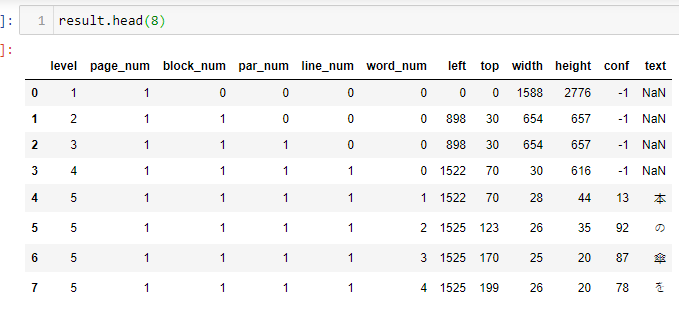
\includegraphics{E:/Users/Usuario/Documents/GitHub_Website/website/japanese_dictionaries/outputs/documents/figure11.png}
\textbf{Figure 11}

From figure 11, we can observe that the output in the column
\textbf{level} generates five levels. Those are pages, blocks,
paragraphs, lines, and words (characters). Each one is subsets of the
previous one.

\hypertarget{page}{%
\subsubsection{Page}\label{page}}

For this example, the page resembles the concept of region, which is the
largest area of the image enclosing all recognized characters. Figure 12
illustrates the page area.

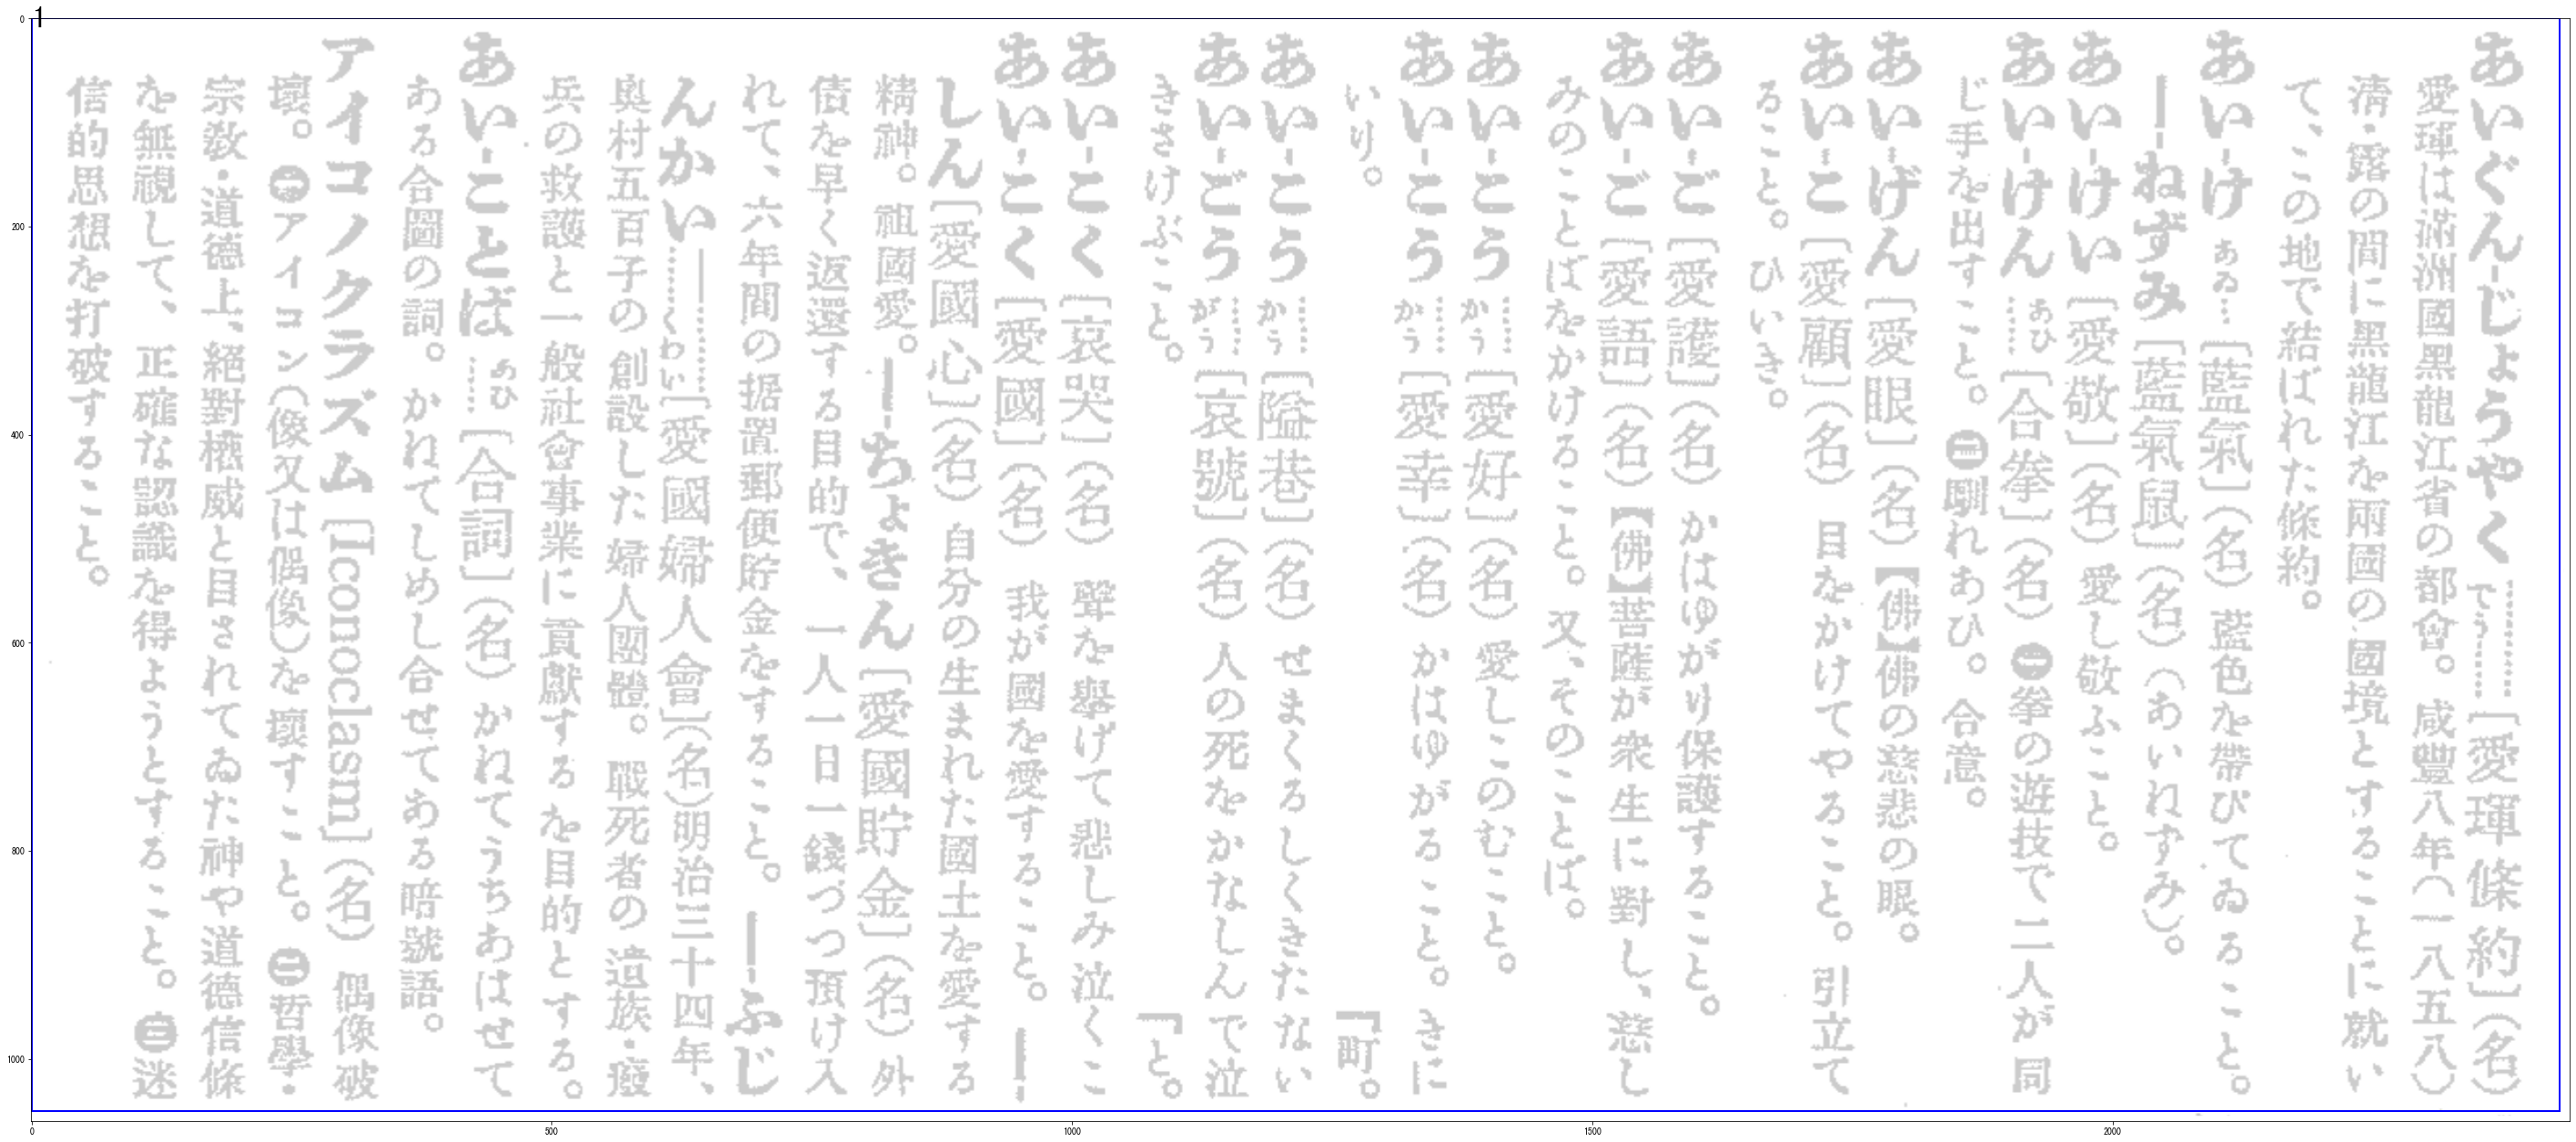
\includegraphics{E:/Users/Usuario/Documents/GitHub_Website/website/japanese_dictionaries/outputs/documents/pytesseract-images/page.png}
\textbf{Figure 12}

\hypertarget{blocks}{%
\subsubsection{Blocks}\label{blocks}}

The blocks are subsets of the page area that consist of small groups of
recognized characters. In figure 13, we can see that most of the blocks
are well ordered. In terms of correctness of the boundaries, we can see
that some of them overlap several characters that are not recognized by
the library.

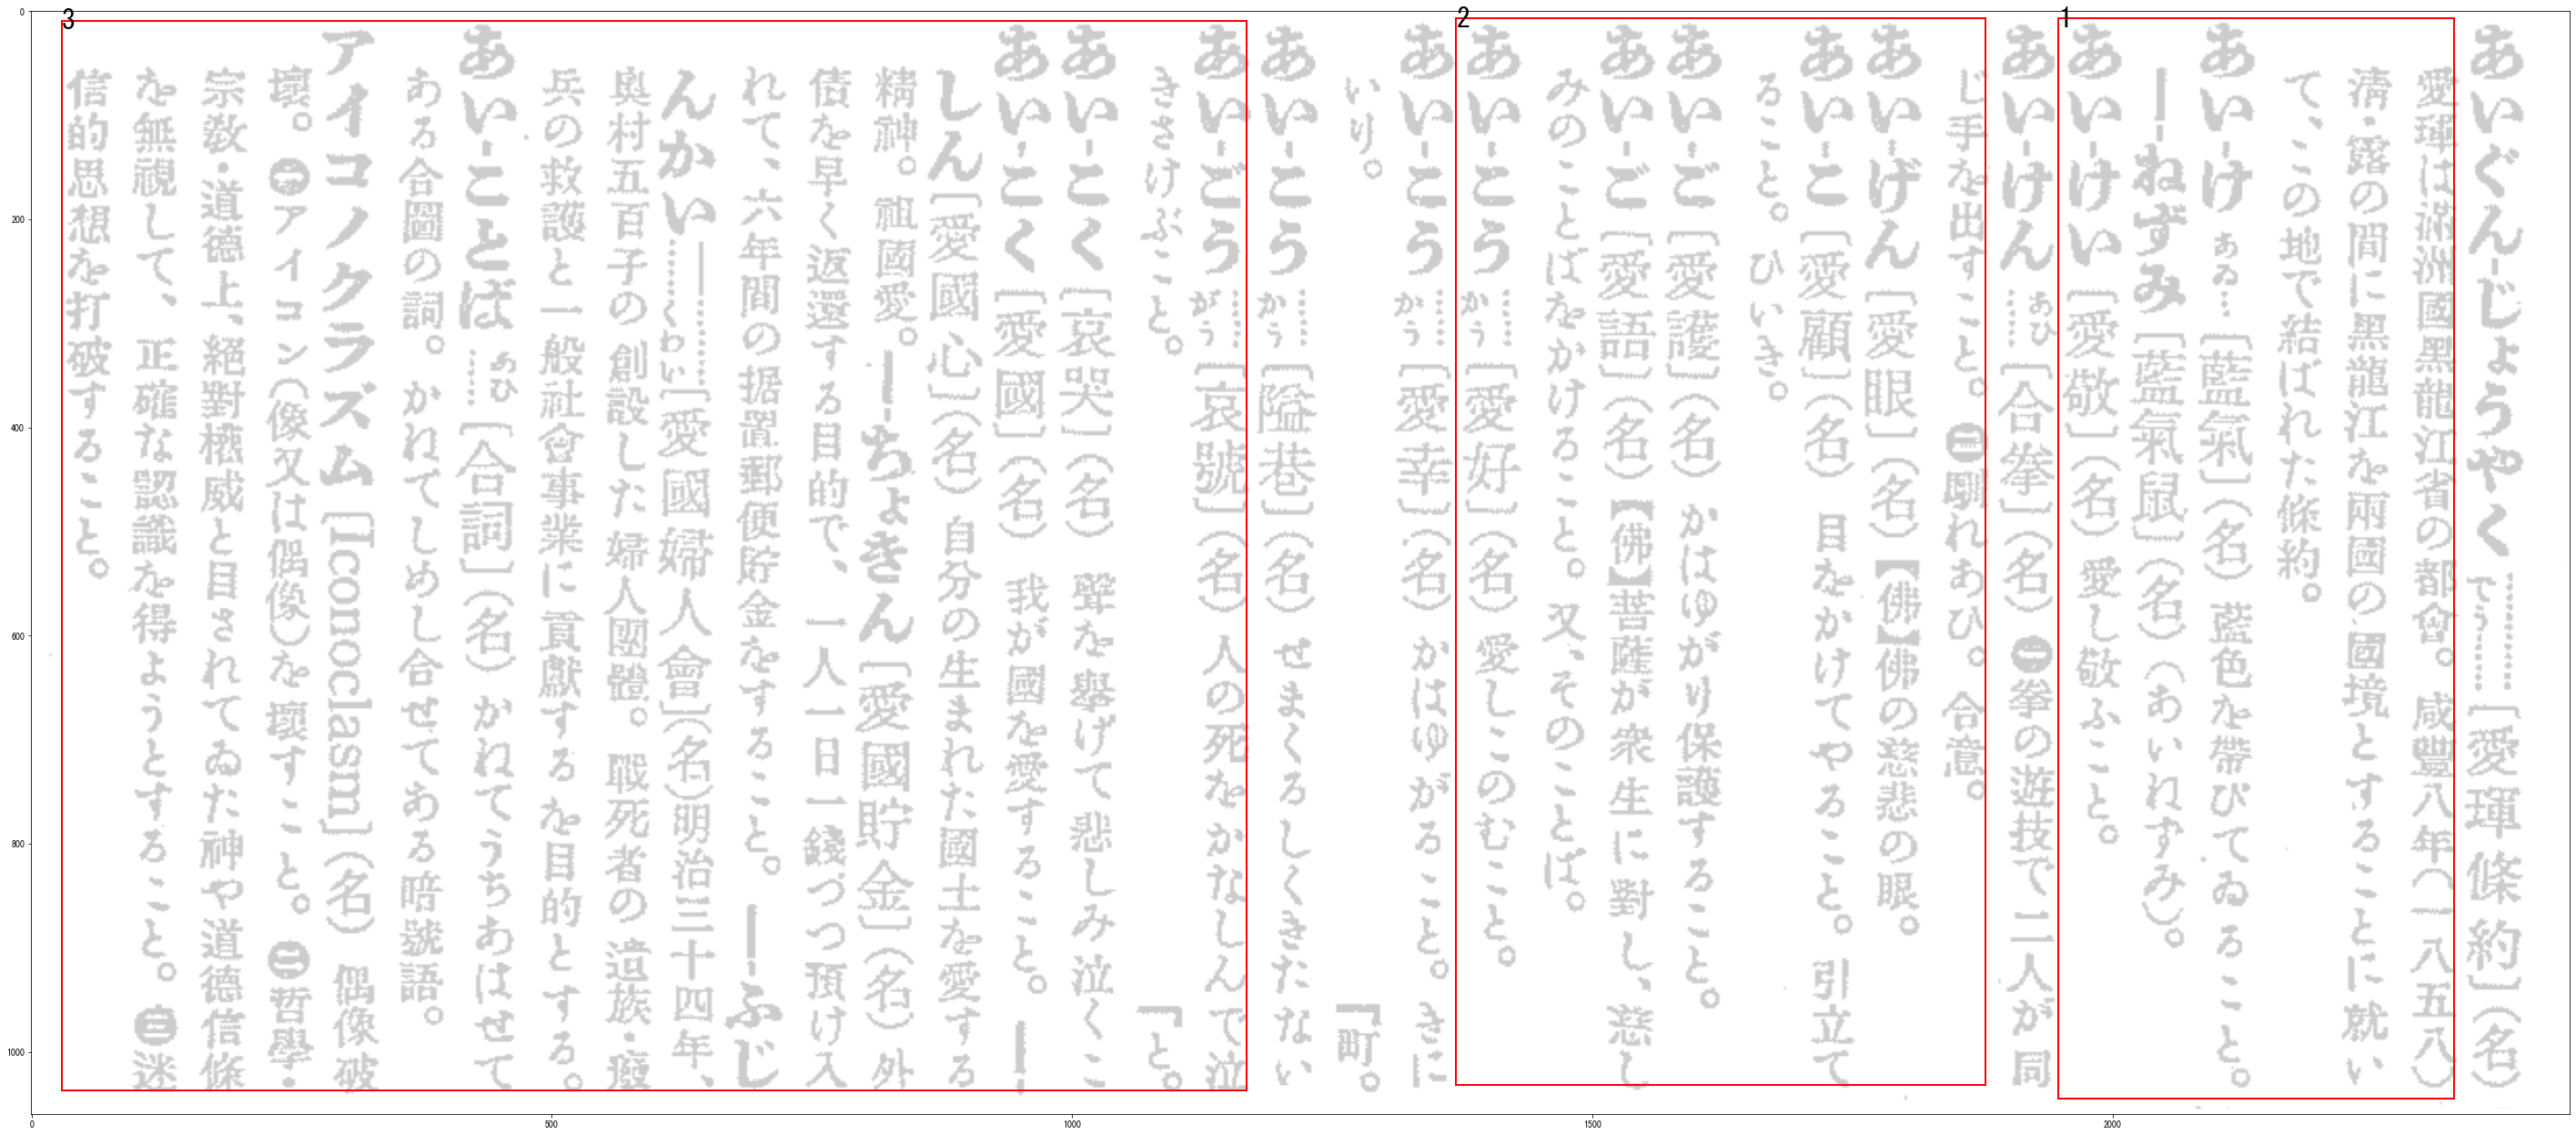
\includegraphics{E:/Users/Usuario/Documents/GitHub_Website/website/japanese_dictionaries/outputs/documents/pytesseract-images/blocks.png}
\textbf{Figure 13}

\hypertarget{paragraphs}{%
\subsubsection{Paragraphs}\label{paragraphs}}

Similar to the blocks, the paragraphs are subsets of blocks. These
follow the same idea of subareas containing a set of characters. In this
case, for example, we can look at paragraphs five and six, which are
subsets of block five. It is interesting to see how the only paragraph
(21) of block 12 is a smaller area compared to the block. This situation
happens in several other blocks. See figure 14 for a better
understanding.

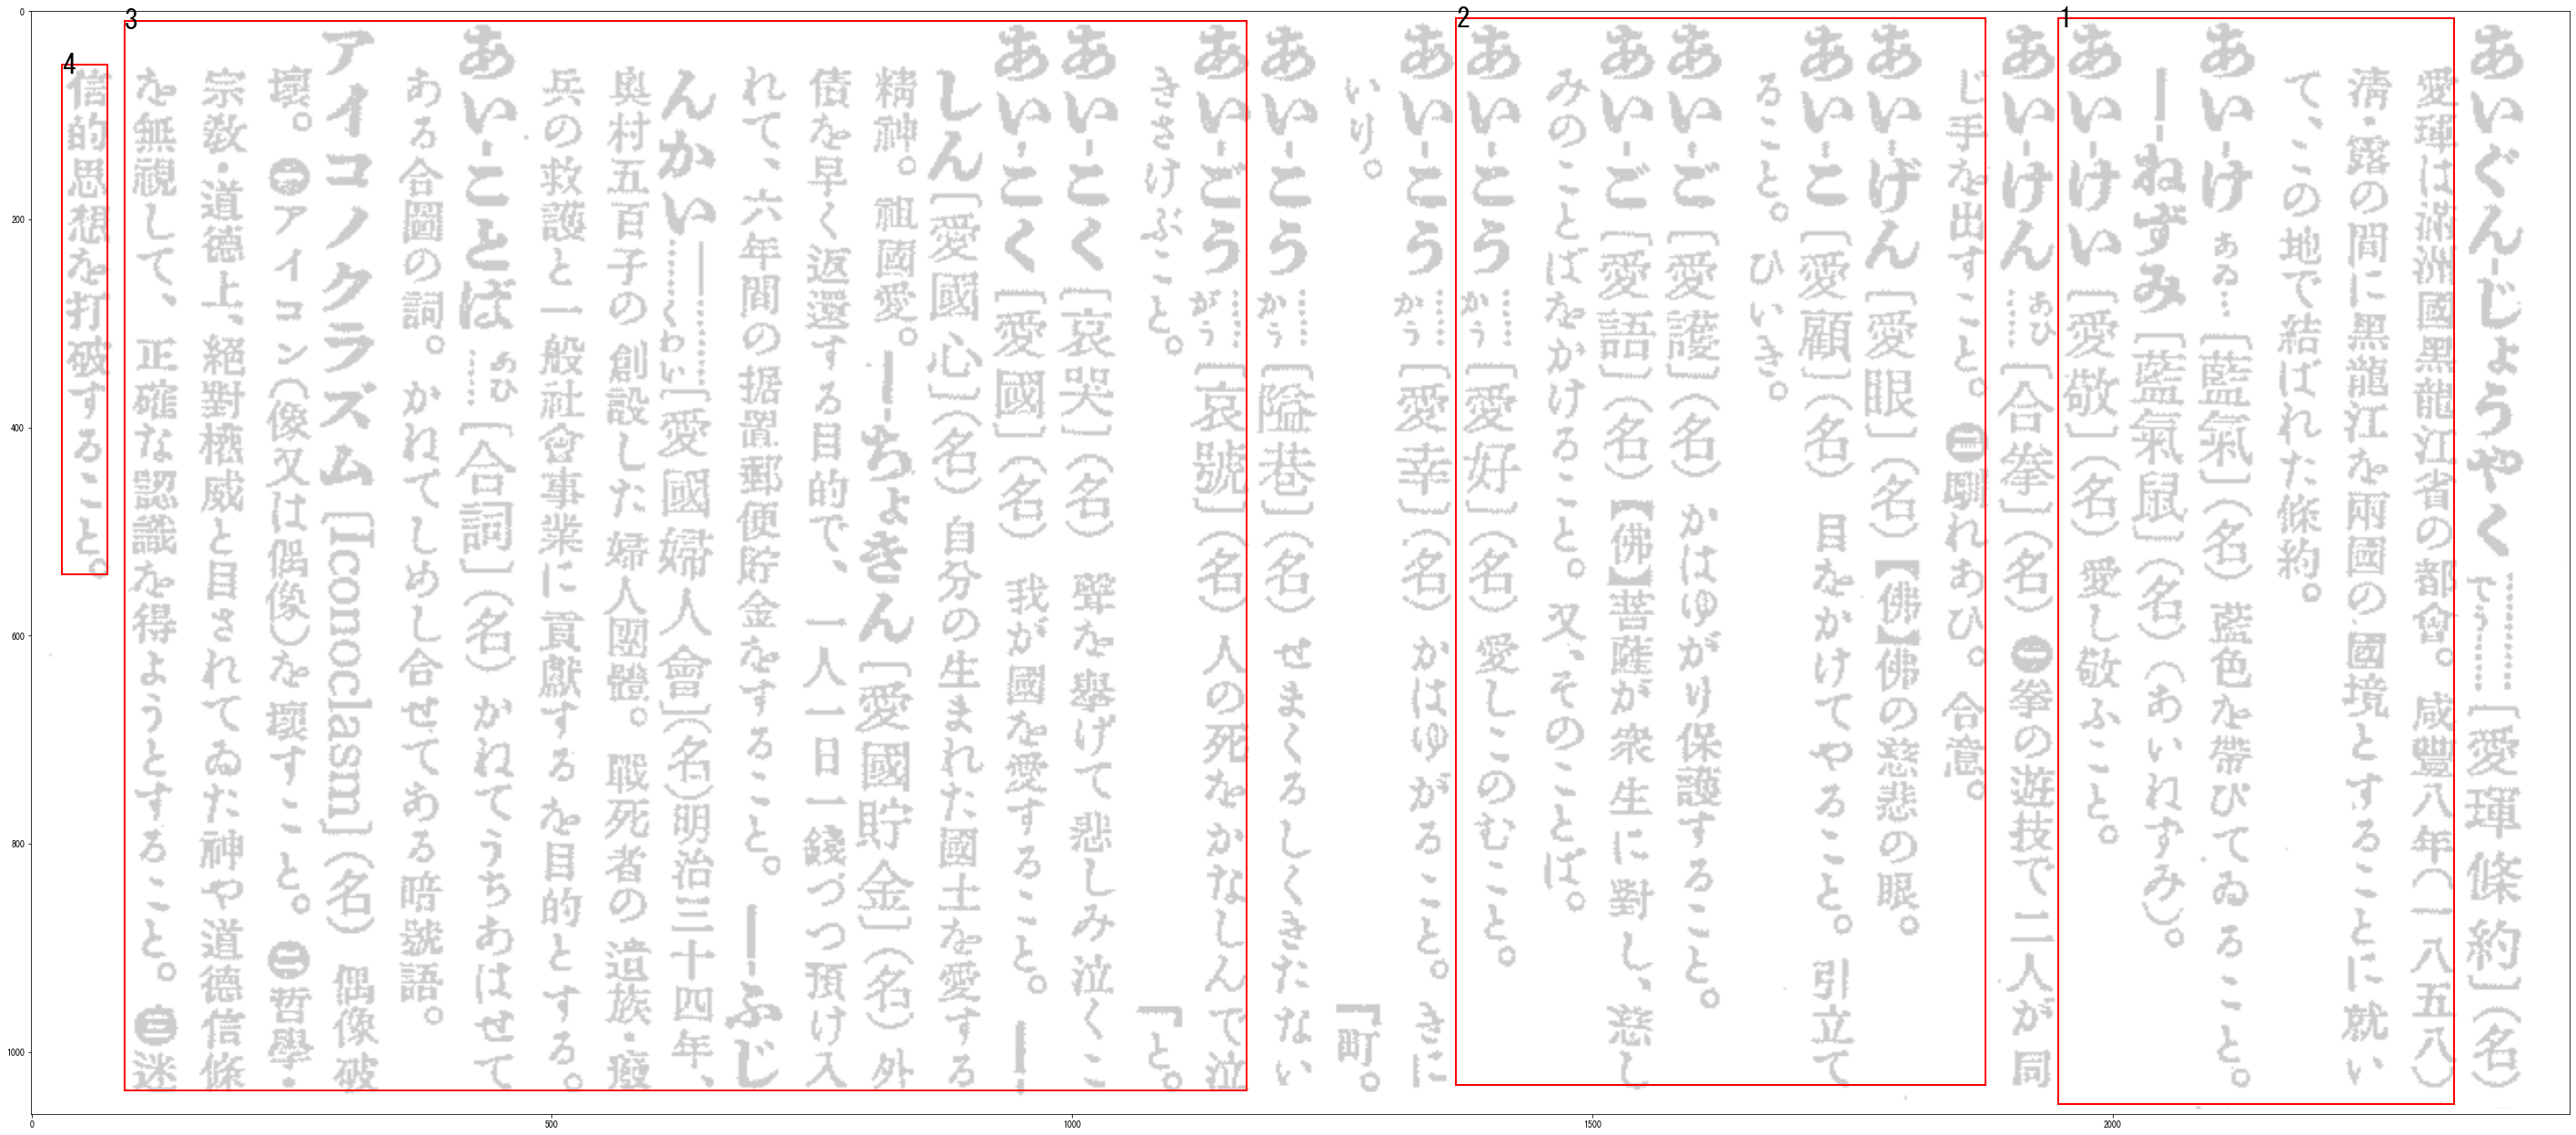
\includegraphics{E:/Users/Usuario/Documents/GitHub_Website/website/japanese_dictionaries/outputs/documents/pytesseract-images/paragraphs.png}
\textbf{Figure 14}

\hypertarget{lines-1}{%
\subsubsection{Lines}\label{lines-1}}

Once the paragraphs are defined, the library provides in figure 15, the
last subsets of characters called Lines. From the example, we can see
that most of the characters are located in one of the lines. However,
several others are not. Some of those cases are curious since there is
no clear reason why those characters are not included. For instance,
between the lines 65 and 66, two clear lines are not recognized by the
library.

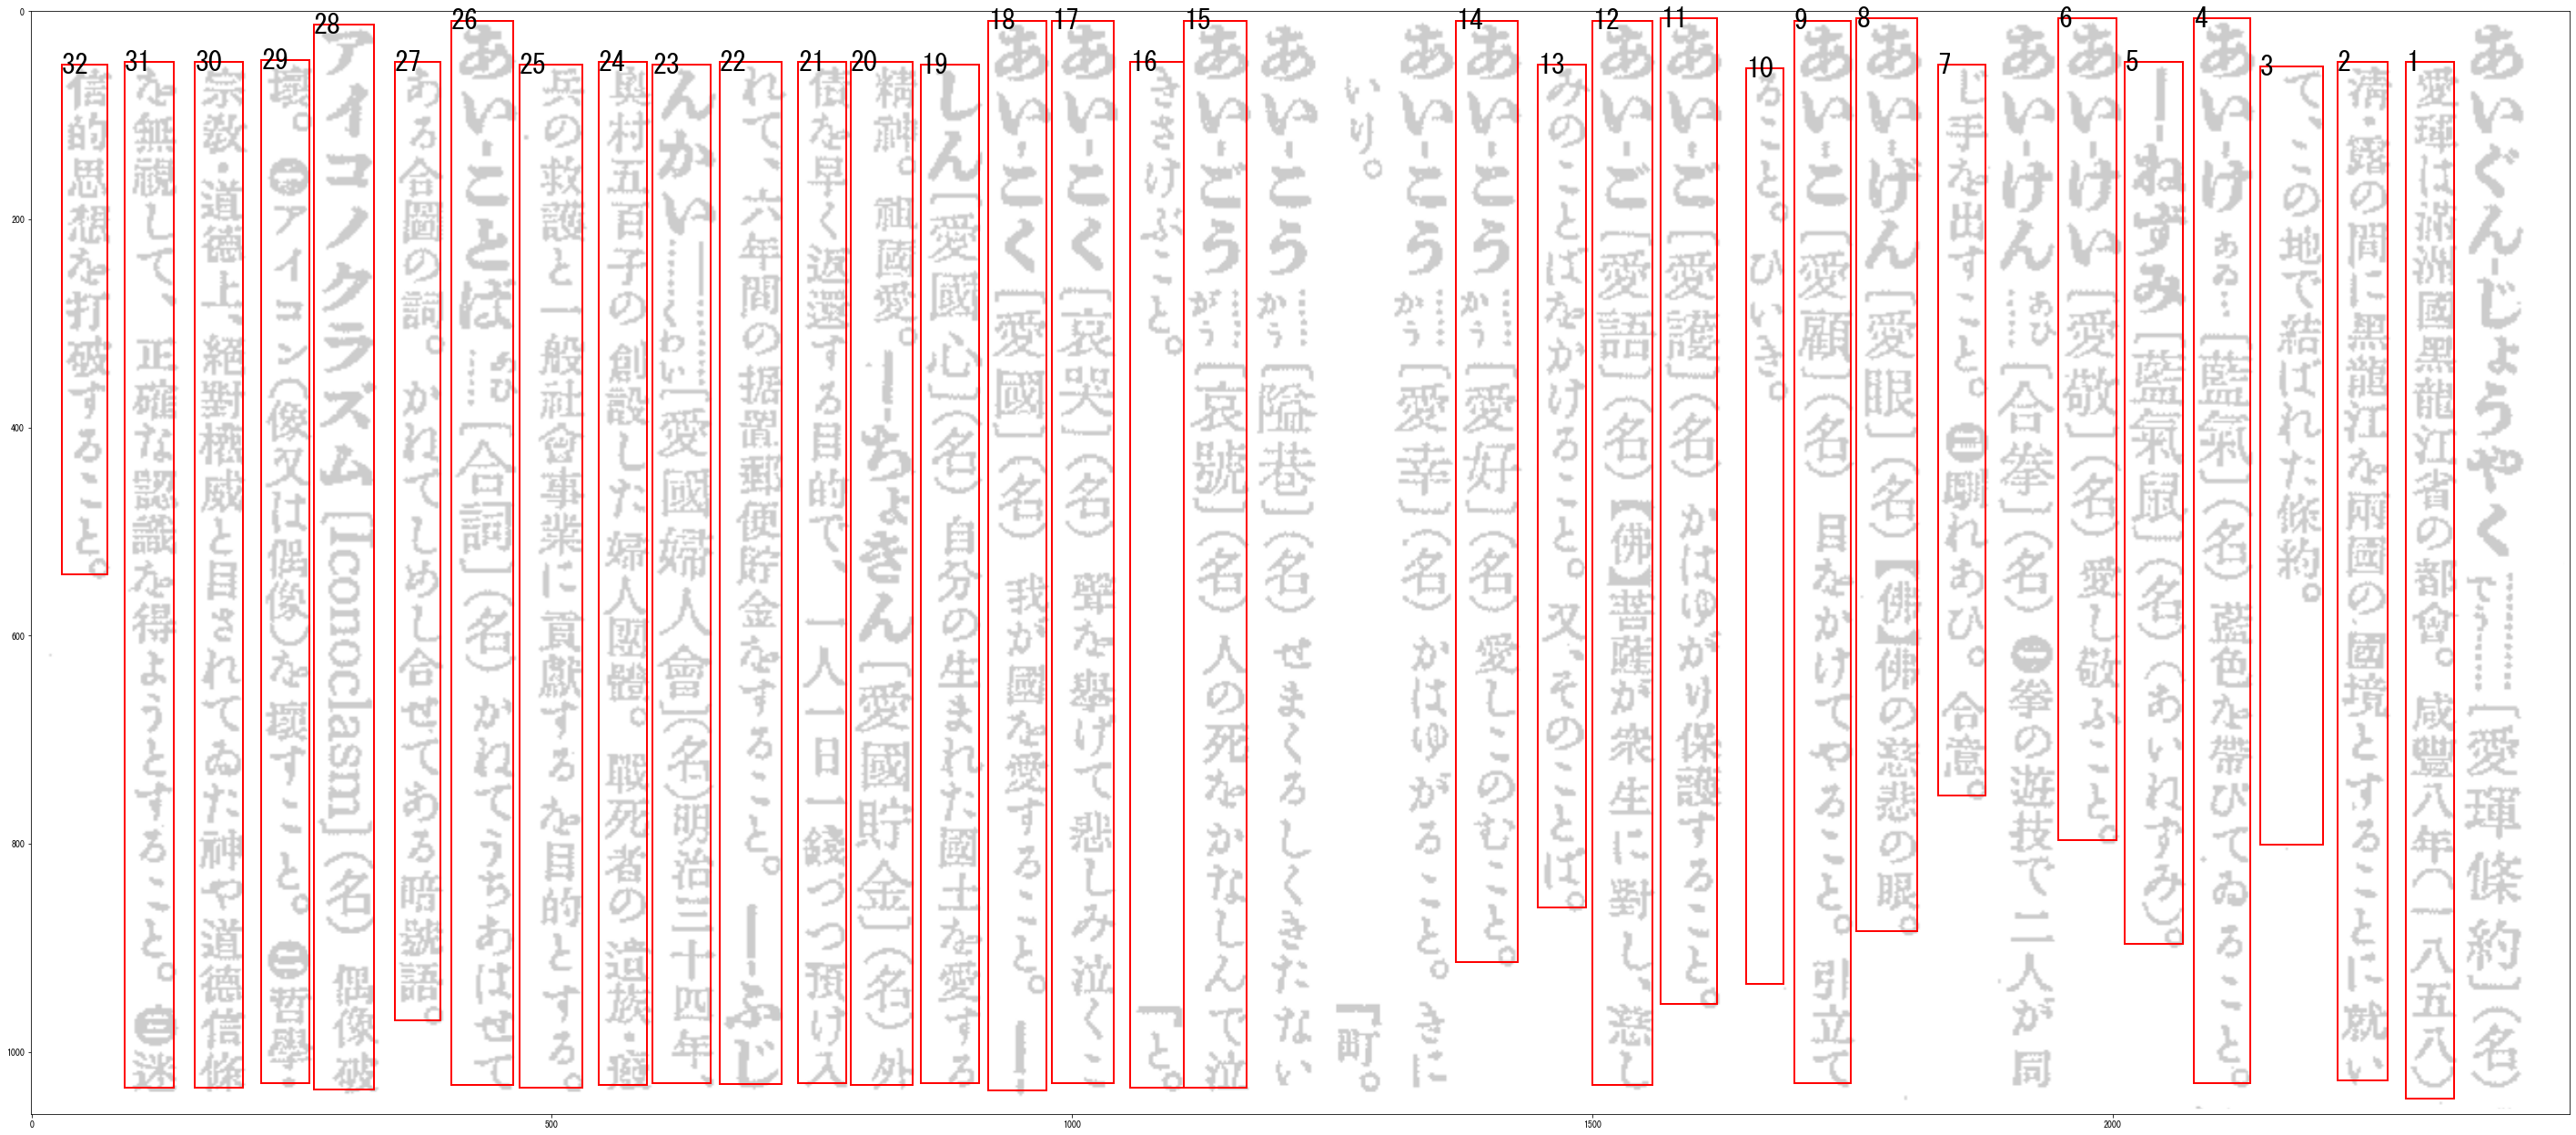
\includegraphics{E:/Users/Usuario/Documents/GitHub_Website/website/japanese_dictionaries/outputs/documents/pytesseract-images/lines.png}\\
\textbf{Figure 15}

\hypertarget{character-boundaries}{%
\subsubsection{Character Boundaries}\label{character-boundaries}}

These boundaries enclose the characters. Figure 16 shows that a
character boundary can include one or more characters. However, some
character boundaries overlap with other ones. Moreover, the same as the
previous areas, several characters have been skipped with no apparent
reason.

\includegraphics{E:/Users/Usuario/Documents/GitHub_Website/website/japanese_dictionaries/outputs/documents/pytesseract-images/boundaries.png}\\
\textbf{Figure 16}

\hypertarget{characters-2}{%
\subsubsection{Characters}\label{characters-2}}

In terms of character-level recognition, we can observe that many
characters are not recognized. Interestingly those characters are in a
correct block, paragraph, line, and character boundary, but it was
skipped. For example, in the first line and the first character boundary
of this line, there are two words, but one of them is not recognized.
Figure 17 illustrates this case.

\includegraphics{E:/Users/Usuario/Documents/GitHub_Website/website/japanese_dictionaries/outputs/documents/pytesseract-images/characters.png}\\
\textbf{Figure 17}

\hypertarget{advantages-and-disadvantages-2}{%
\subsubsection{Advantages and
Disadvantages}\label{advantages-and-disadvantages-2}}

\hypertarget{advantages-2}{%
\paragraph{Advantages}\label{advantages-2}}

The most important advantage is that this is a free library. It is also
a wrapper from Google's Tesseract Engine. Moreover, the way it presents
the covered areas are very detailed. It offers blocks, paragraphs,
lines, boundaries, and finally the character level.

\hypertarget{disadvantages-2}{%
\paragraph{Disadvantages}\label{disadvantages-2}}

Some lines were completely ignored by Pyteseract, even thought it was
clear enough to be recognized by the tool.

\hypertarget{kindai-ocr}{%
\subsection{Kindai-OCR}\label{kindai-ocr}}

According to the Center for Open Data in the Humanities, Kindai-OCR is
an OCR system for modern Japanese documents. It was built under the N2I
project that study state-of-the-art statistical models for OCR, and work
on the development of infrastructure and providing open access to data.
The datasets were constructed by the University of Tokyo Center for
Education and Research and the National Institute of Japanese Language
and are used for OCR machine learning. These datasets are commonly known
as the Modern Magazine Datasets.

The Kindai-OCR code was developed in Python and released as an open
source code in August 2020 on Github..The Github folder contains all the
necessary code and instructions to assess the OCR tool. \textbf{{[}not
sure if it is necessary to mention the modification in the file test.py,
in order to run the model using GPUs.{]}}

After running the Kindai-OCR for our samples, the system generated three
outputs. They are explained as follows:

\hypertarget{file-result.xml}{%
\subsubsection{File result.xml}\label{file-result.xml}}

This file is presented in an Extensible Markup Language (XML) format
containing a tree with the identified lines, as well as the
corresponding characters. An example of the is shown as follows:

\begin{verbatim}
<?xml version='1.0' encoding='Shift_JIS'?>
<paper xmlns="http://codh.rois.ac.jp/modern-magazine/"><page dpi="100" file="00-sample_pages_3_sec_3.png" height="1040" number="1" width="2430"><line height="905" width="72" x="332" y="0">あいくるし發路事、愛くるし(形、</line><line height="1026" width="76" x="466" y="0">あいくち島(合巳。名。あれせも。ものよ</line><line height="1026" width="69" x="592" y="0">あいくすりし((きき」名その人の爲に信身あ</line><line height="1031" width="65" x="660" y="0">あいきん(及兵」(名起しい得をうつし表しした</line><line height="1031" width="78" x="778" y="0">あいきん愛心。名客する東なふする、</line><line height="361" width="72" x="849" y="0">あいきよう對</line><line height="292" width="64" x="918" y="0">あいきよう</line><line height="1031" width="64" x="981" y="0">あいきよう對(愛婦(名(((らきささ。((彼。。</line><line height="292" width="64" x="2264" y="0">あいきまう</line><line height="997" width="69" x="1749" y="34">(愛教商)名」名毎金。造。。愛もがなてては立</line><line height="337" width="55" x="286" y="38">府がはゆらしい。</line><line height="930" width="68" x="407" y="38">くあふ人。○つばのない兌。。ヒ直。九五五五。</line>
\end{verbatim}

\hypertarget{kraken---python-library}{%
\subsection{Kraken - Python Library}\label{kraken---python-library}}

Kraken is a python library created by Benjamin Kiessling from Université
PSL in France and Leipzig University. This library is a combination of a
fork (independent development built on an existing one) from the Ocropus
package and CLSTM neural network library. Its purpose was to improve
accuracy and performance rates compared with Ocropus. It has been tested
with languages such as Arabic, Persian, Syriac Polytonic Greek, Latin,
among other. However, there is no information about japanese-trained
models.

To assess the performance of this library, it is necessary to train a
model for japanese texts. To do that, Kraken offers a function called
\textbf{train}. This function expects a series of images that according
to Kraken´s website, these images must be high quality scans, preferably
color or grayscale, and at least 300dpi. Images in PDF format are not
allowed. Each image must be accompanied with a text file with extension
.gt.txt. This file will contain the character(s) that corresponds to the
image with the same name. For instance in figure xx we see the image
file is called \textbf{sec1\_line1.png}, the pair-wise text element for
this image is \textbf{sec\_line.gt.txt}.

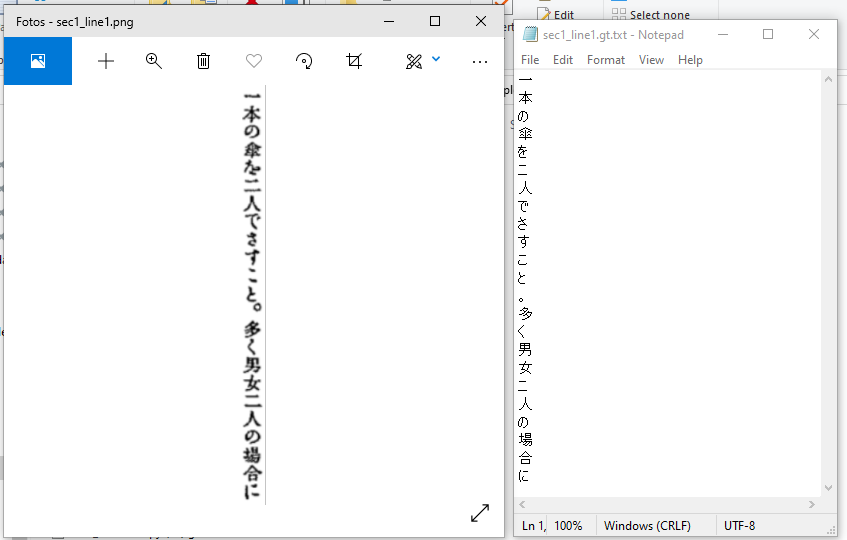
\includegraphics{E:/Users/Usuario/Documents/GitHub_Website/website/japanese_dictionaries/outputs/documents/figure18.png}\\
\textbf{Figure 18}

After the training stage, Kraken analyses the layout and extracts text
lines from an input image for later processing by the recognition. A
step by step process is provided by Kraken´s website
(\url{http://kraken.re/index.html}) to recognize text from an image
using the model we want.

\hypertarget{training-process-challenges}{%
\subsubsection{Training process
challenges}\label{training-process-challenges}}

The training process itself is very friendly. However, the data
preparation is the most important part as it generates the samples we
feed into the model. Other studies pointed out that for languages such
as Arabic, at least 800 lines are required to train a descent model. For
the Japanese text of this study we trained 36 lines in which several
characters appear more than once. The result after the training process
was not good, indicating that the need of greater sample data might be
needed which is not in the scope of this study.

\hypertarget{other-limitations}{%
\section{Other limitations}\label{other-limitations}}

In order to use this library it is required to have either Linux or Mac.
In this study, we use Google Colab which is offers a Linux environment
to assess the library.

\hypertarget{amazon-textract}{%
\subsection{Amazon Textract}\label{amazon-textract}}

According to Amazon's website, Amazon Textract can detect Latin-script
characters from the standard English alphabet and ASCII symbols.

\url{https://aws.amazon.com/textract/faqs/}

\hypertarget{amazon-rekognition}{%
\subsection{Amazon Rekognition}\label{amazon-rekognition}}

According to Amazon's website, Amazon Rekognition supports text in most
Latin scripts and numbers. Text detection recognizes up to 50 sequences
of characters per the image or video frame and lists them as words and
lines.

\url{https://aws.amazon.com/rekognition/faqs/}

\hypertarget{evaluation}{%
\section{Evaluation}\label{evaluation}}

For each option, we rank them based on two scales: results and
difficulty. We need to work out a definition for each of these.

Diego's comment: From what I learned so far, it could be easiness (an
API is more straightforward than a library), number of characters
correctly recognized, flexibility (the opposite of easiness), and cost.
Moreover, some APIs such as Google's groups more than one character,
whereas Azure returns only one character per boundary.

In terms of flexibility\ldots{}

Sequence of the characters\ldots{}

Output given\ldots xml, json, flat file, csv\ldots{}

NUmber of characters well recognized\ldots(Accuracy)

The main aspect of the end product will be a graph with two axis, and
dots for where each service is positioned, coloured or faceted by the
test.

\hypertarget{discussion}{%
\section{Discussion}\label{discussion}}

\hypertarget{appendix}{%
\section{Appendix}\label{appendix}}

\hypertarget{references}{%
\section{References}\label{references}}

1:
\url{https://www.researchgate.net/publication/267465115_An_Overview_and_Applications_of_Optical_Character_Recognition}

2:
\url{https://books-scholarsportal-info.myaccess.library.utoronto.ca/en/read?id=/ebooks/ebooks2/wiley/2011-12-13/1/9780470176535}

3:

4:
\url{https://docs.microsoft.com/en-us/azure/cognitive-services/computer-vision/home}

5:
\url{https://docs.microsoft.com/en-us/azure/cognitive-services/computer-vision/quickstarts/python-print-text}

6: \url{https://cloud.google.com/vision/docs/ocr}

7: \url{https://pypi.org/project/pytesseract/}

8: \url{https://github.com/tesseract-ocr/tessdata}

9: \url{https://github.com/UB-Mannheim/tesseract/wiki}

10: \url{http://codh.rois.ac.jp/software/kindai-ocr/}

11: \url{https://github.com/ducanh841988/Kindai-OCR}

12: Anh Duc Le, Daichi Mochihashi, Katsuya Masuda, Hideki Mima, and Nam
Tuan Ly. 2019. Recognition of Japanese historical text lines by an
attention-based encoder-decoder and text line generation. In Proceedings
of the 5th International Workshop on Historical Document Imaging and
Processing (HIP '19). Association for Computing Machinery, New York, NY,
USA, 37--41. \url{DOI:https://doi.org/10.1145/3352631.3352641}

\end{document}
